% Apéndice: manual de usuario.
% Capturas en imagenes/manual/, recortadas sin barra de estado ni barra de navegación (945 x 1871 px).

\chapter{Manual de usuario}
\label{ap:manual}

\captionsetup[sub]{font=scriptsize}

\newcommand{\manualhueco}{\hspace{0.02\textwidth}}

Quiet Companion se usa desde dos móviles. En el de la persona mayor está el asistente con el que conversa; en el de un familiar, si ella lo desea, un panel desde el que la acompaña a distancia. Este manual explica cada parte por separado: la sección~\ref{sec:manual-mayor} está pensada para la persona mayor o para quien la ayude a empezar, y la sección~\ref{sec:manual-familiar}, para el familiar. La aplicación necesita un móvil Android 7.0 o posterior con conexión a Internet.

\section{La persona mayor}
\label{sec:manual-mayor}

\subsection{Primeros pasos}

\begin{figure}[!htb]\centering
  \begin{subfigure}[t]{0.165\textwidth}\centering
    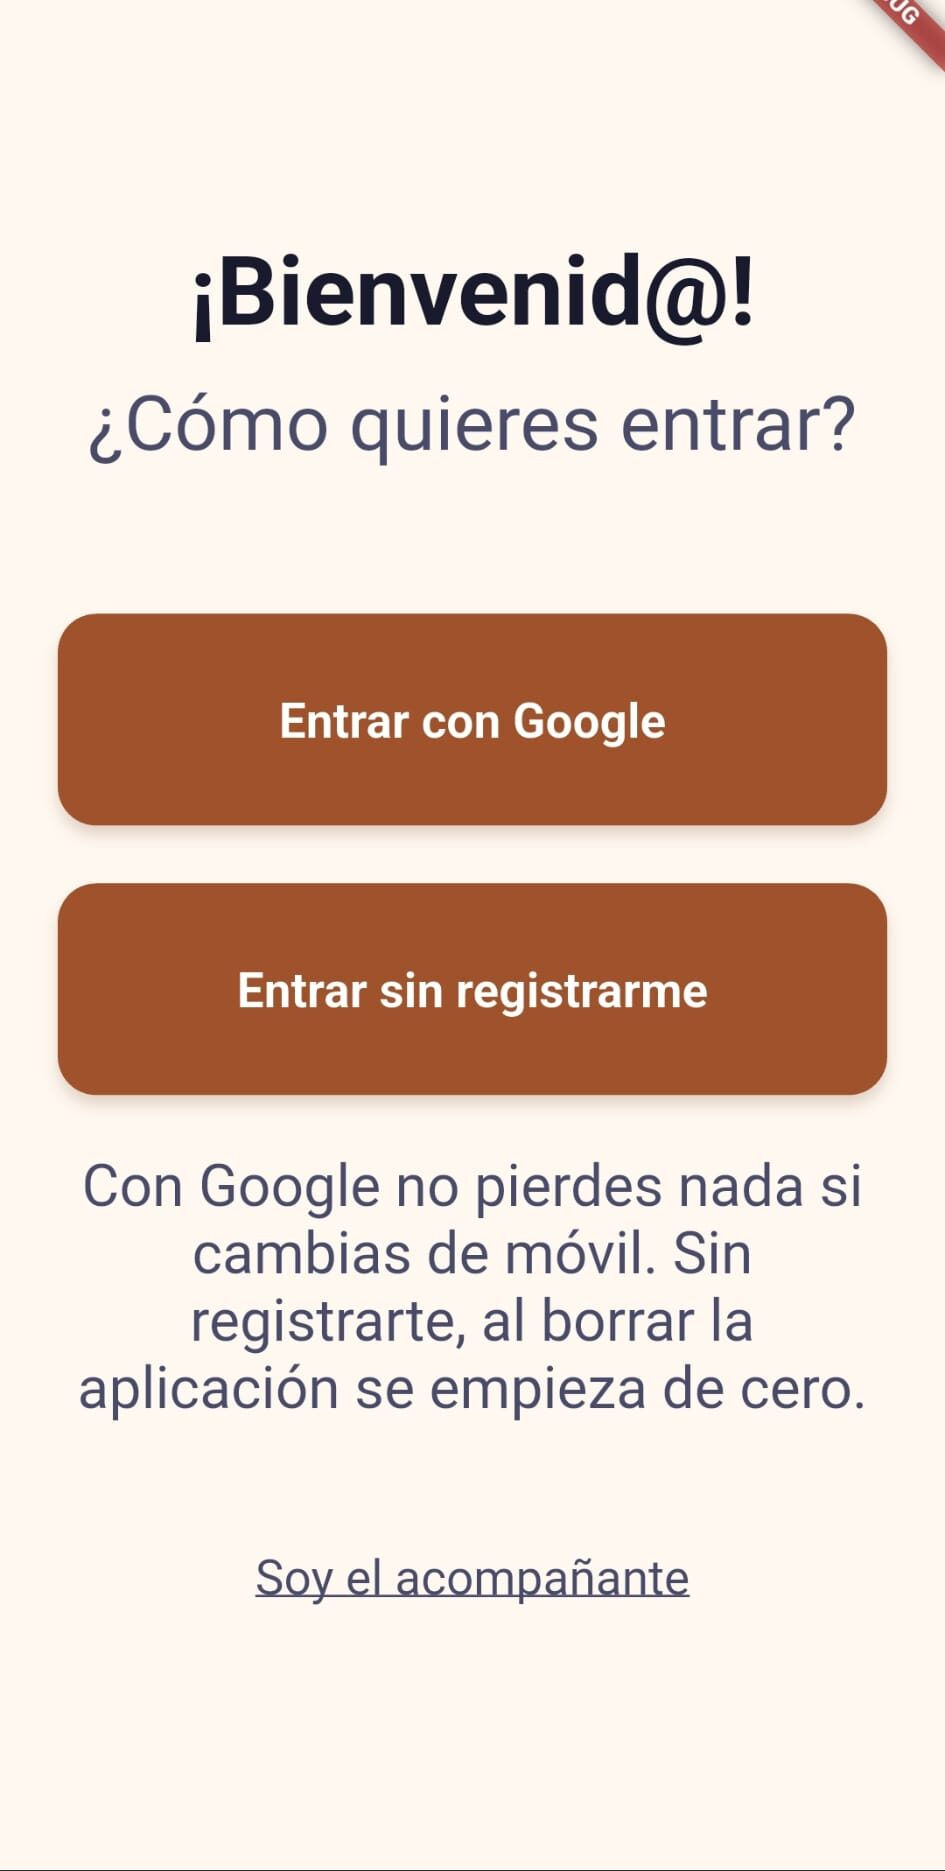
\includegraphics[width=\linewidth]{imagenes/manual/mayor-entrar}
    \caption{Entrar}
  \end{subfigure}\manualhueco
  \begin{subfigure}[t]{0.165\textwidth}\centering
    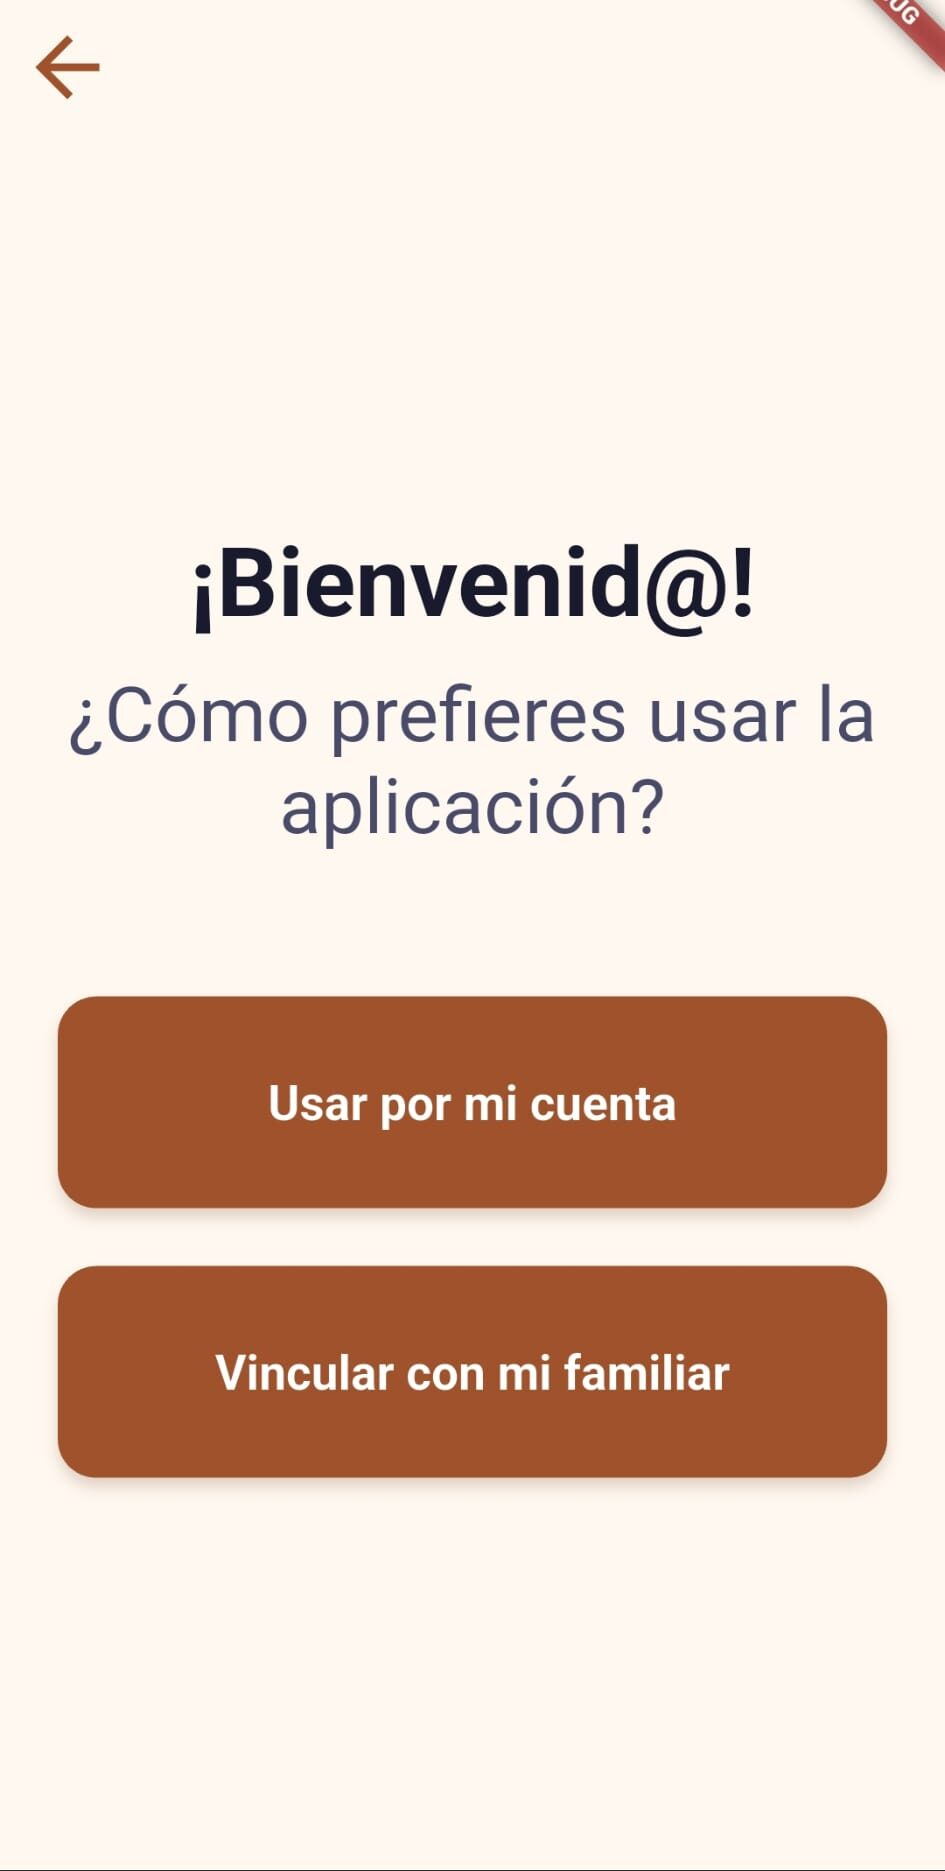
\includegraphics[width=\linewidth]{imagenes/manual/mayor-modo}
    \caption{Modo de uso}
  \end{subfigure}\manualhueco
  \begin{subfigure}[t]{0.165\textwidth}\centering
    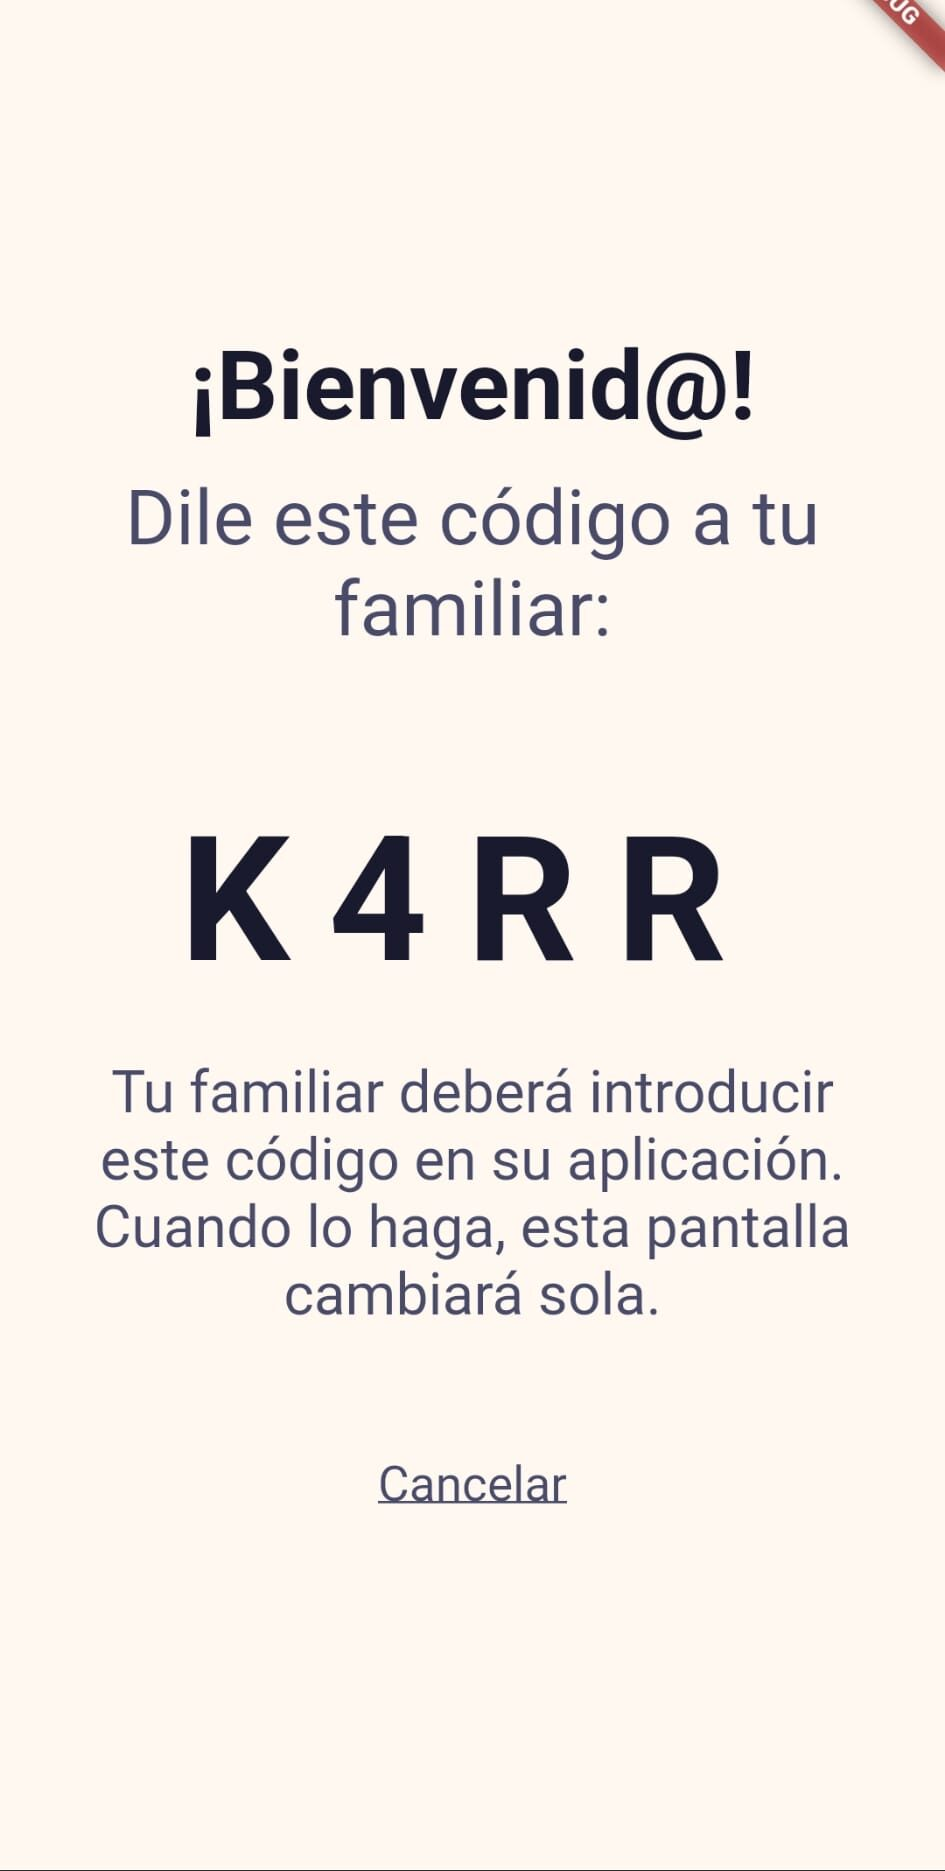
\includegraphics[width=\linewidth]{imagenes/manual/mayor-codigo}
    \caption{Código}
  \end{subfigure}\manualhueco
  \begin{subfigure}[t]{0.165\textwidth}\centering
    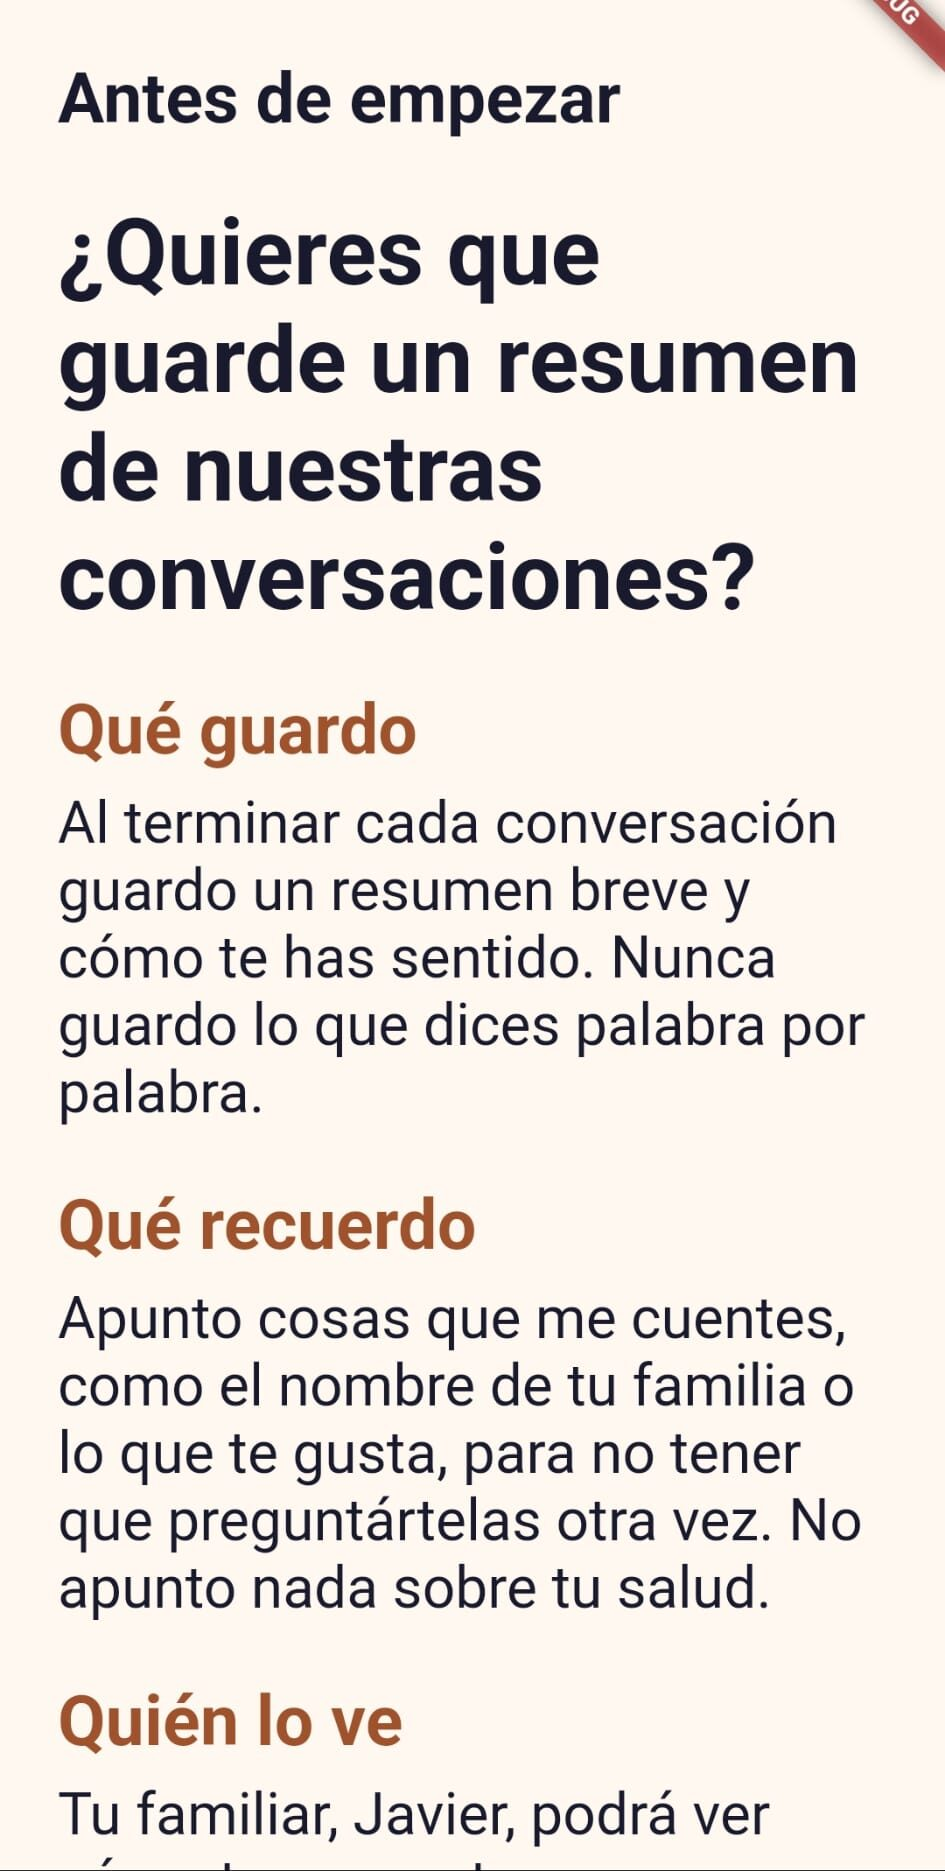
\includegraphics[width=\linewidth]{imagenes/manual/mayor-consentimiento}
    \caption{Pregunta}
  \end{subfigure}\manualhueco
  \begin{subfigure}[t]{0.165\textwidth}\centering
    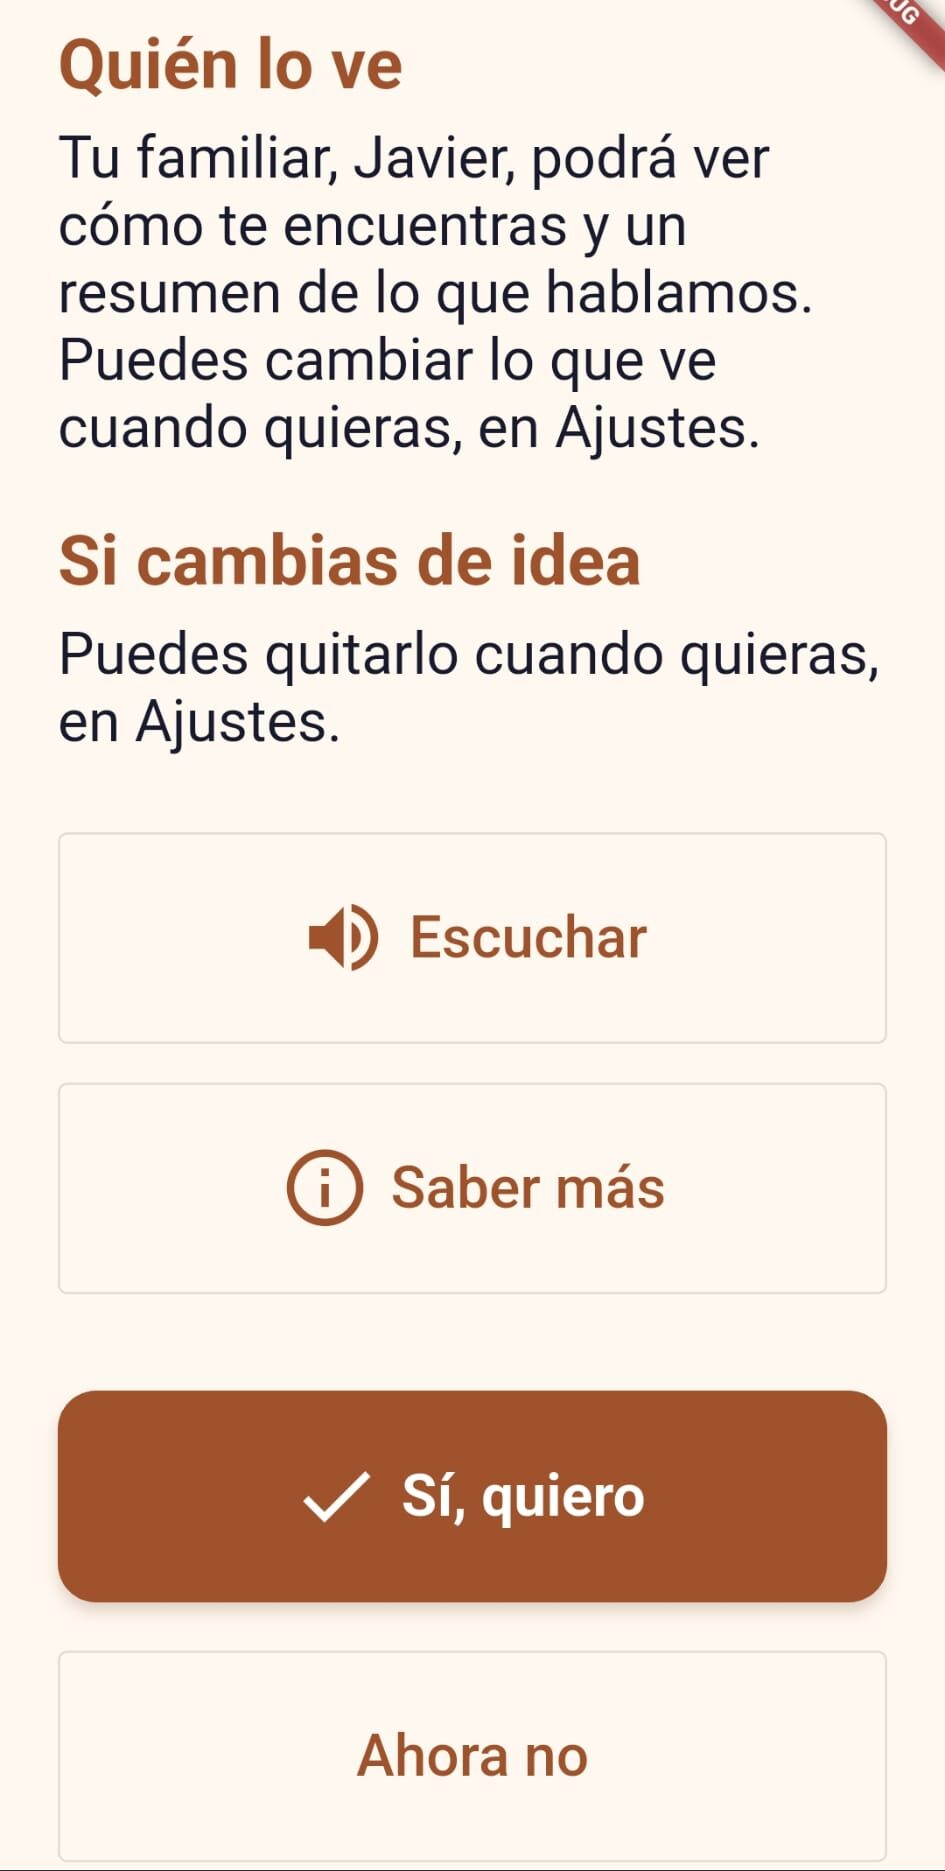
\includegraphics[width=\linewidth]{imagenes/manual/mayor-consentimiento-botones}
    \caption{Respuesta}
  \end{subfigure}
  \caption{Primeros pasos de la persona mayor.}
  \label{fig:manual-inicio}
\end{figure}

La primera vez que abra la aplicación, esta le preguntará cómo quiere entrar (\autoref{fig:manual-inicio}). Con <<Entrar con Google>> conserva todo aunque cambie de móvil; con <<Entrar sin registrarme>> no necesita ninguna cuenta, pero si borra la aplicación empezará de cero. Más adelante puede pasar a su cuenta de Google desde Ajustes. El enlace <<Soy el acompañante>> es para su familiar.

Después elija cómo quiere usarla. Con <<Usar por mi cuenta>> conversa con el asistente sin que nadie más vea nada. Con <<Vincular con mi familiar>> aparece un código de cuatro caracteres: dígaselo a su familiar para que lo escriba en su aplicación. Cuando lo haga, la pantalla cambiará sola.

Por último, el asistente le pregunta si quiere que guarde un resumen de sus conversaciones. La pantalla explica qué se guarda, qué recuerda el asistente y quién puede verlo; <<Escuchar>> se lo lee en voz alta y <<Saber más>> da todos los detalles. Puede contestar <<Sí, quiero>> o <<Ahora no>>. Si no acepta, puede conversar igualmente, pero no se guarda ningún resumen. Lo que conteste puede cambiarlo cuando quiera desde Ajustes.

\subsection{Conversar con el asistente}

\begin{figure}[!htb]\centering
  \begin{subfigure}[t]{0.27\textwidth}\centering
    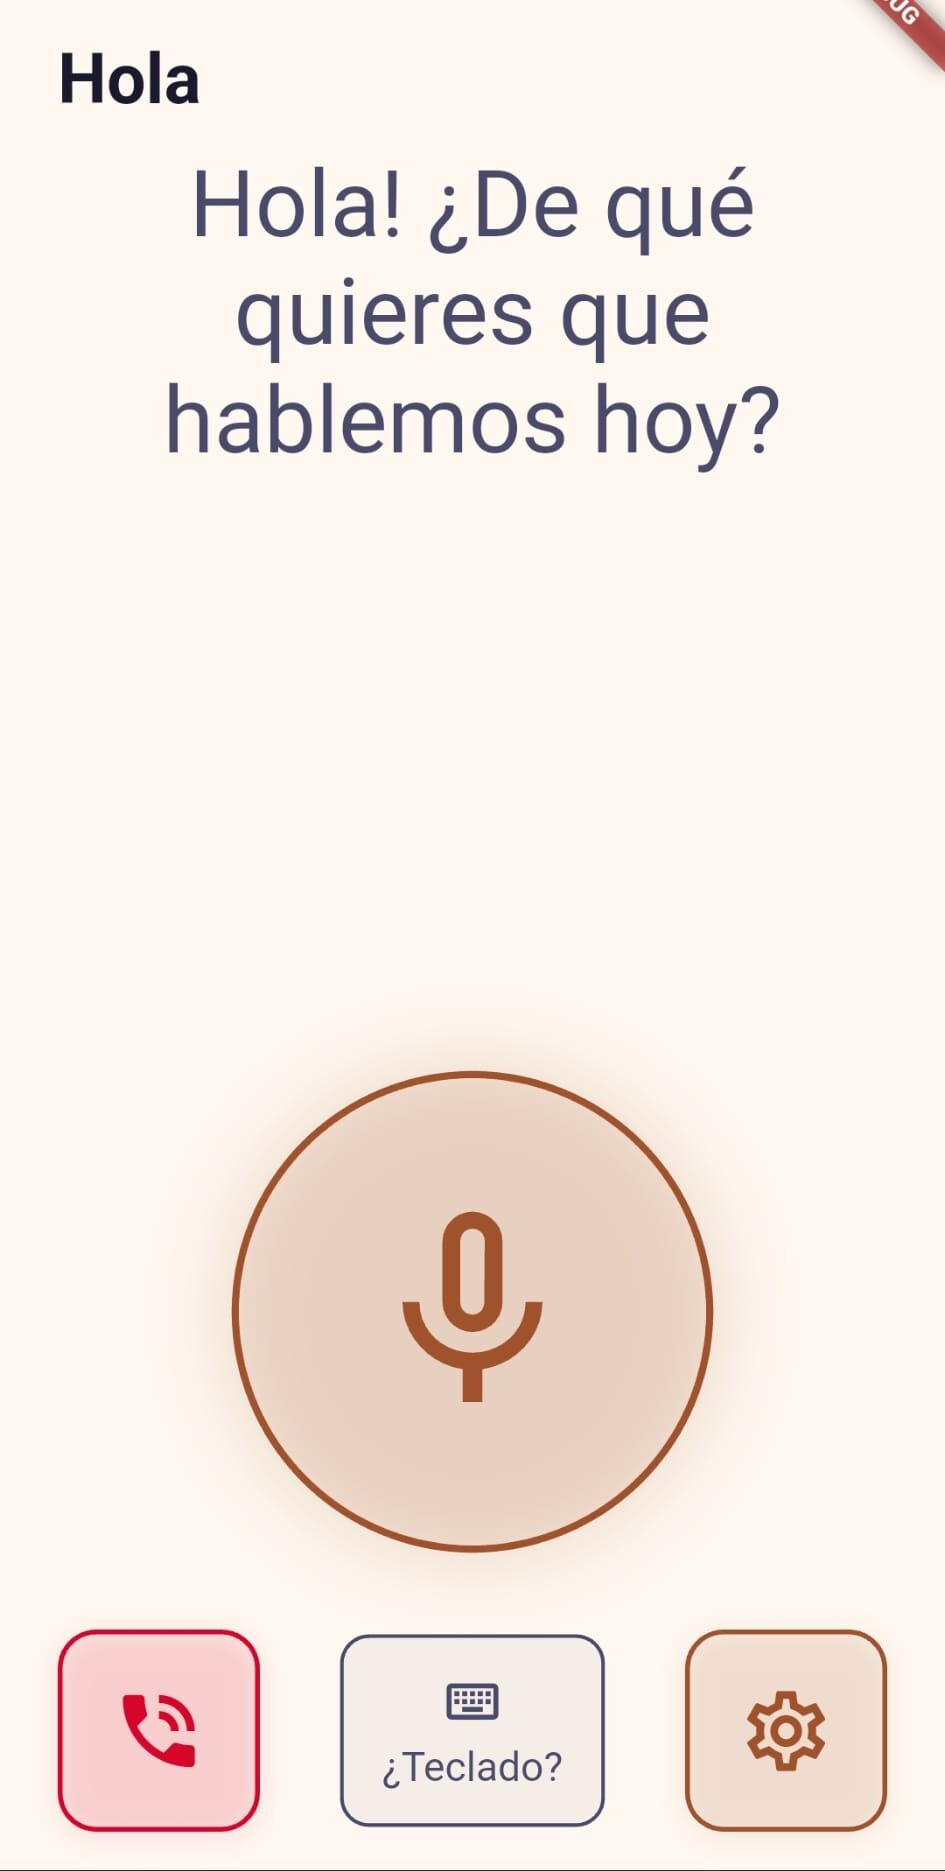
\includegraphics[width=\linewidth]{imagenes/manual/mayor-principal-voz}
    \caption{Pantalla principal}
  \end{subfigure}\hfill
  \begin{subfigure}[t]{0.27\textwidth}\centering
    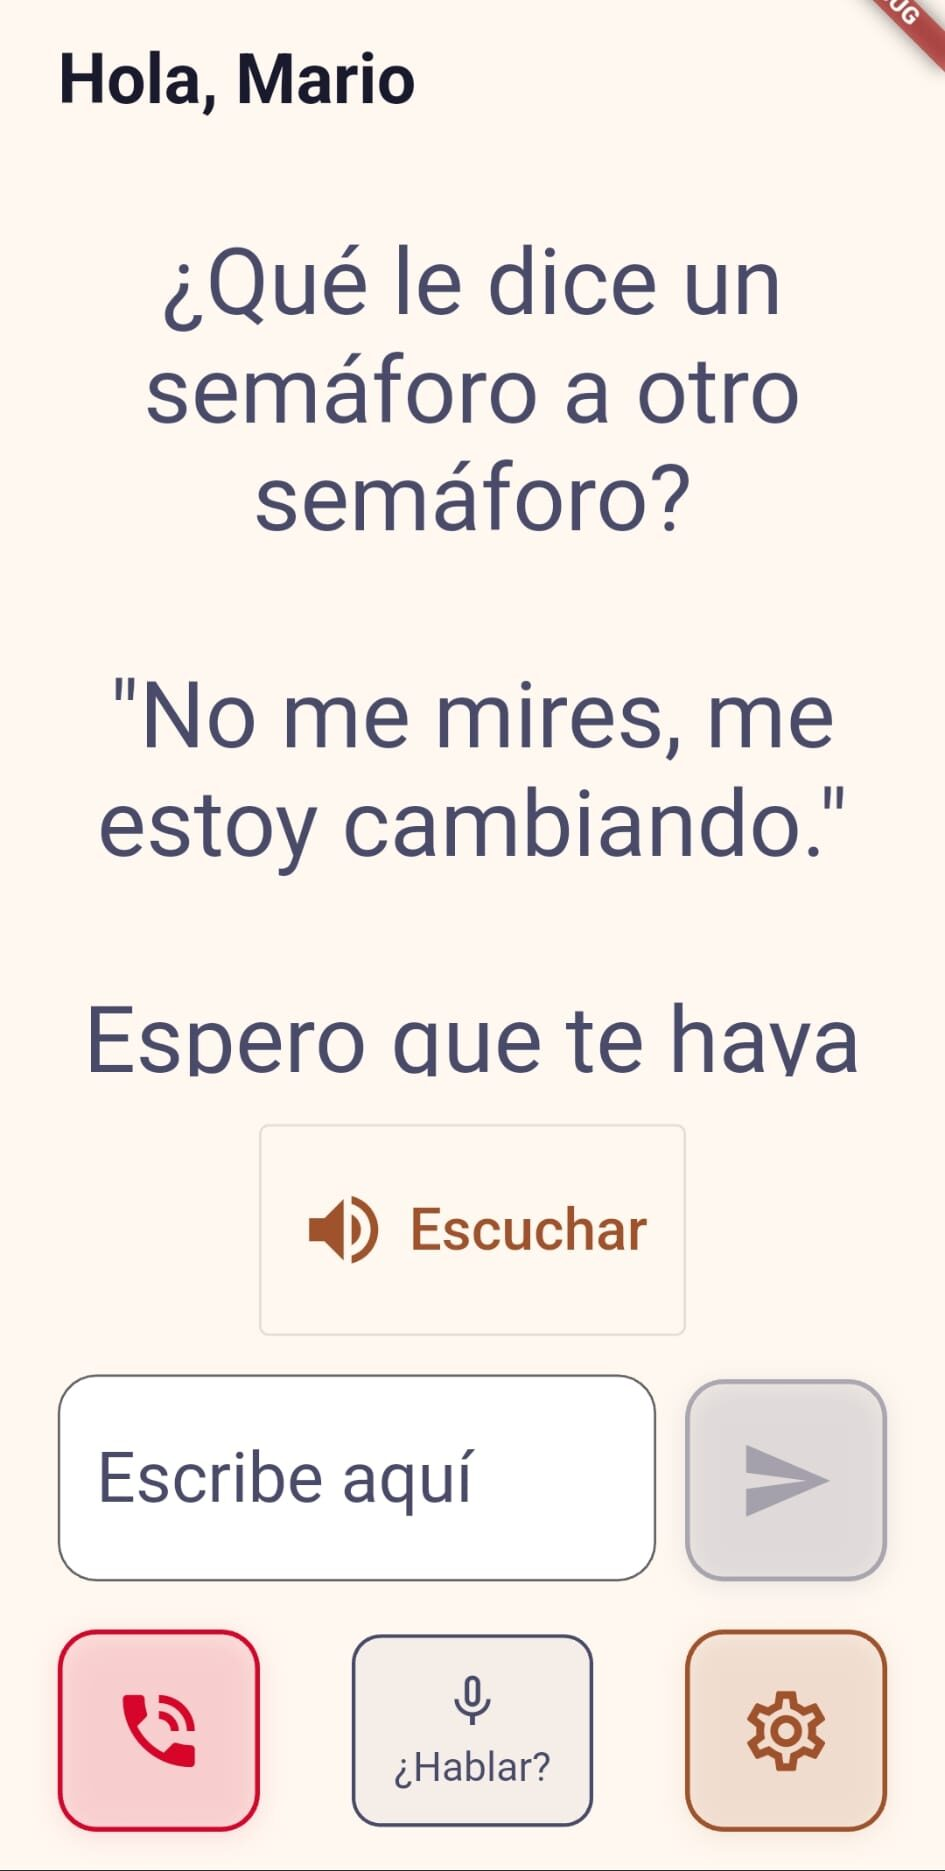
\includegraphics[width=\linewidth]{imagenes/manual/mayor-principal-teclado}
    \caption{Modo teclado}
  \end{subfigure}\hfill
  \begin{subfigure}[t]{0.27\textwidth}\centering
    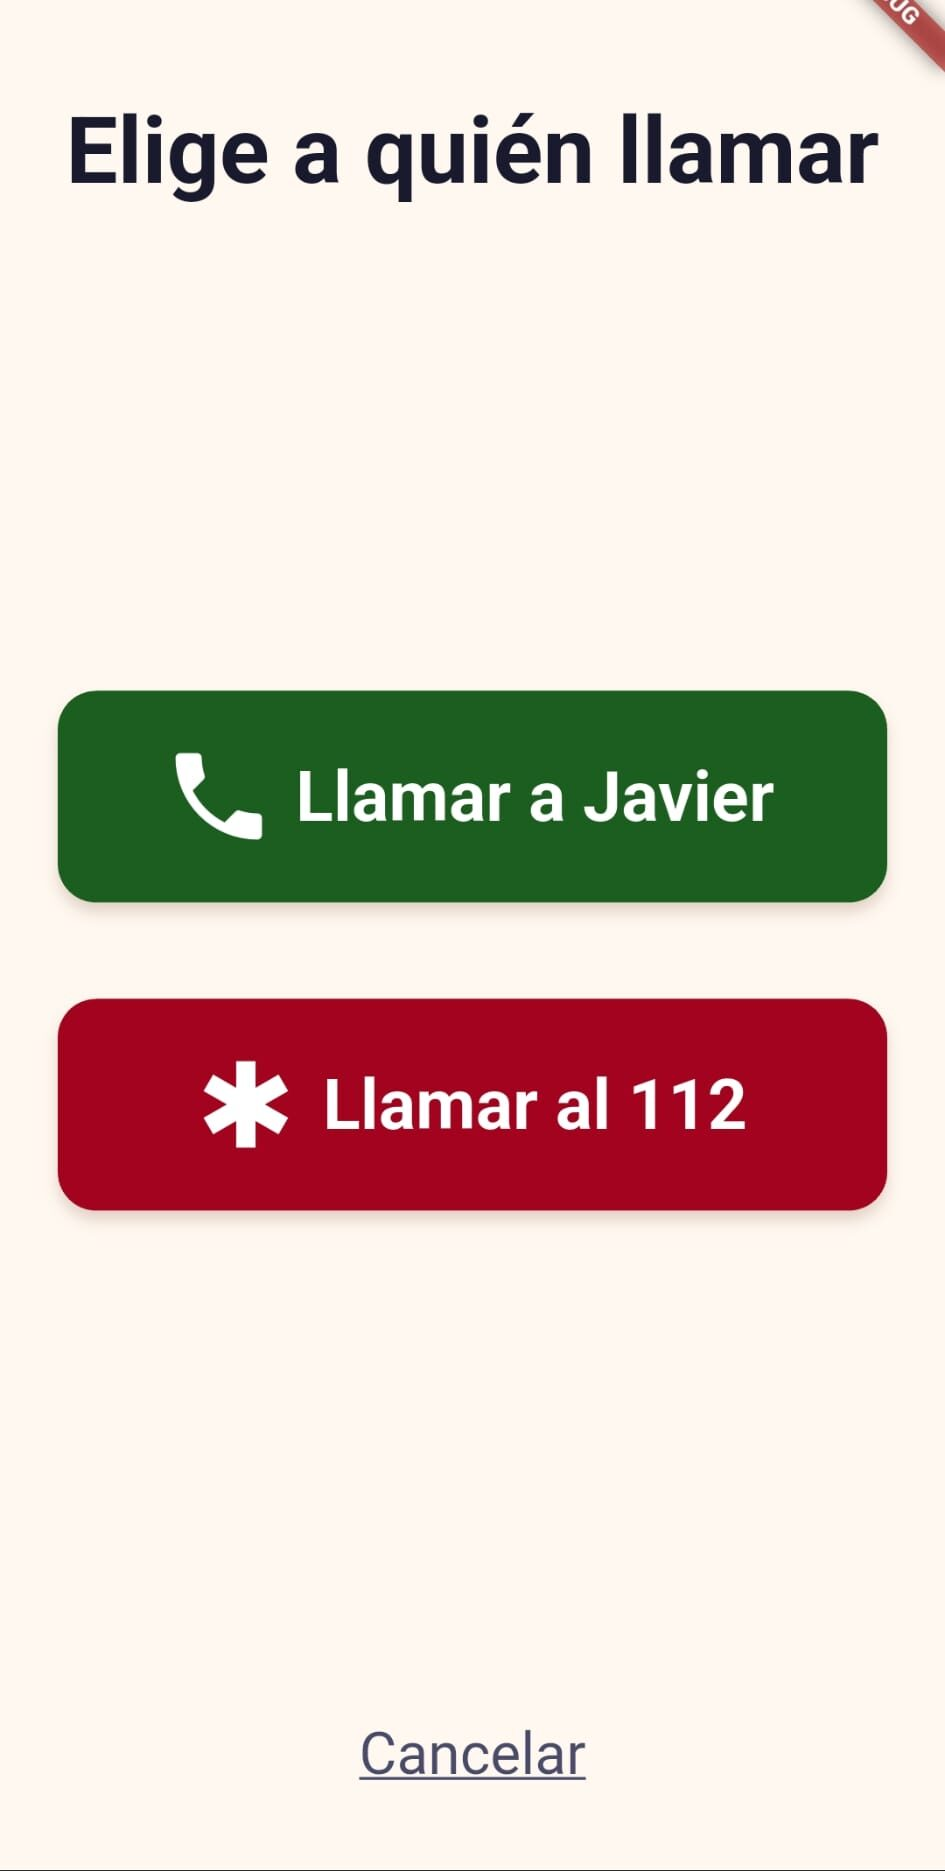
\includegraphics[width=\linewidth]{imagenes/manual/mayor-emergencia}
    \caption{Emergencia}
  \end{subfigure}
  \caption{Conversación y llamada de emergencia.}
  \label{fig:manual-principal}
\end{figure}

La pantalla principal tiene un solo botón grande, el del micrófono (\autoref{fig:manual-principal}). Tóquelo y hable con normalidad. Cuando se quede en silencio unos segundos, el asistente entiende que ha terminado y le contesta en voz alta; si no quiere esperar, toque otra vez el micrófono al acabar de hablar. Para seguir la conversación, vuelva a tocarlo. Si el asistente le corta antes de que termine, alargue el <<Tiempo que te espero>> en Ajustes.

También puede escribir. Toque <<¿Teclado?>>, escriba en el recuadro <<Escribe aquí>> y pulse la flecha de enviar. En este modo la respuesta no se lee sola: toque <<Escuchar>> para oírla. <<¿Hablar?>> vuelve al micrófono.

Abajo hay siempre tres botones: el teléfono rojo, para pedir ayuda; el del centro, para cambiar entre voz y teclado; y la rueda, para los ajustes. Cuando ya hay alguna conversación resumida, aparece además el botón <<Mi semana>> (apartado~\ref{sec:manual-mi-semana}).

\subsection{Pedir ayuda}

El botón rojo del teléfono abre la pantalla de emergencia. <<Llamar a>>, seguido de un nombre, llama a su familiar o a su contacto de emergencia, y <<Llamar al 112>> llama a emergencias. El móvil abre el marcador con el número ya escrito y solo queda pulsar el botón de llamar. <<Cancelar>> vuelve a la conversación.

Si está vinculado, su contacto de emergencia es su familiar; si usa la aplicación por su cuenta, elíjalo en Ajustes, dentro de <<Mis datos>>. El asistente no avisa a nadie por sí solo: si necesita ayuda, use siempre este botón.

\subsection{Ajustes}

\begin{figure}[!htb]\centering
  \begin{subfigure}[t]{0.165\textwidth}\centering
    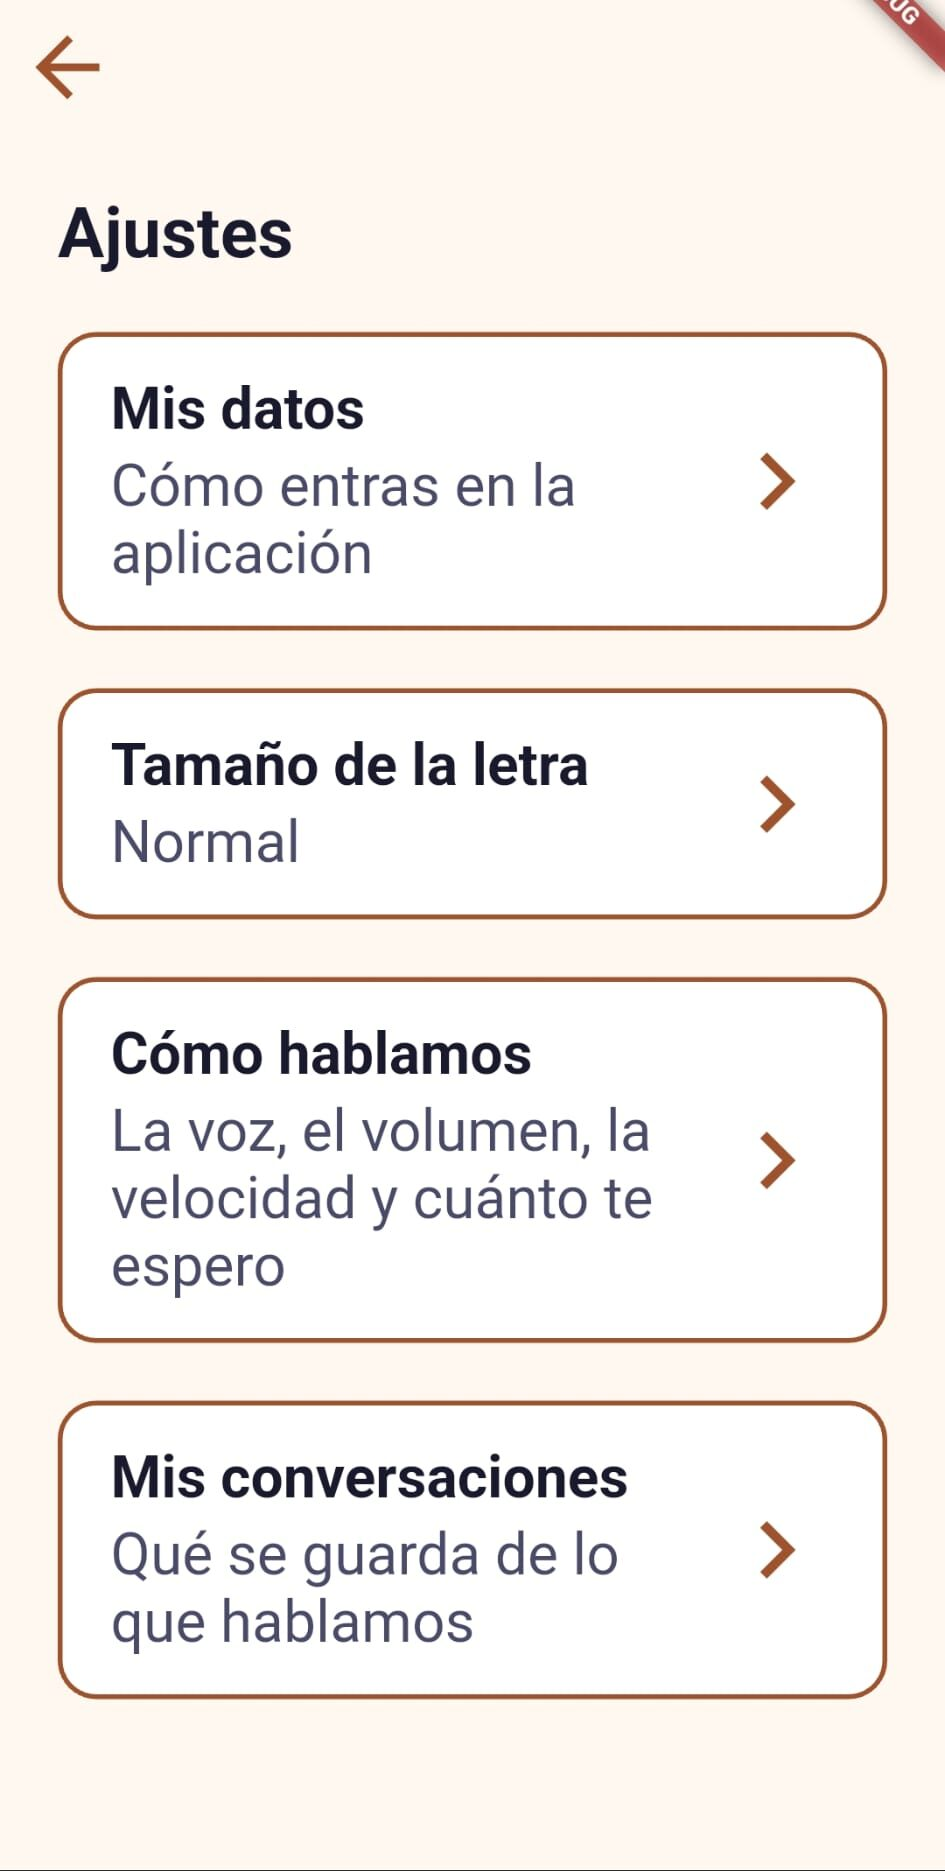
\includegraphics[width=\linewidth]{imagenes/manual/mayor-ajustes}
    \caption{Ajustes}
  \end{subfigure}\manualhueco
  \begin{subfigure}[t]{0.165\textwidth}\centering
    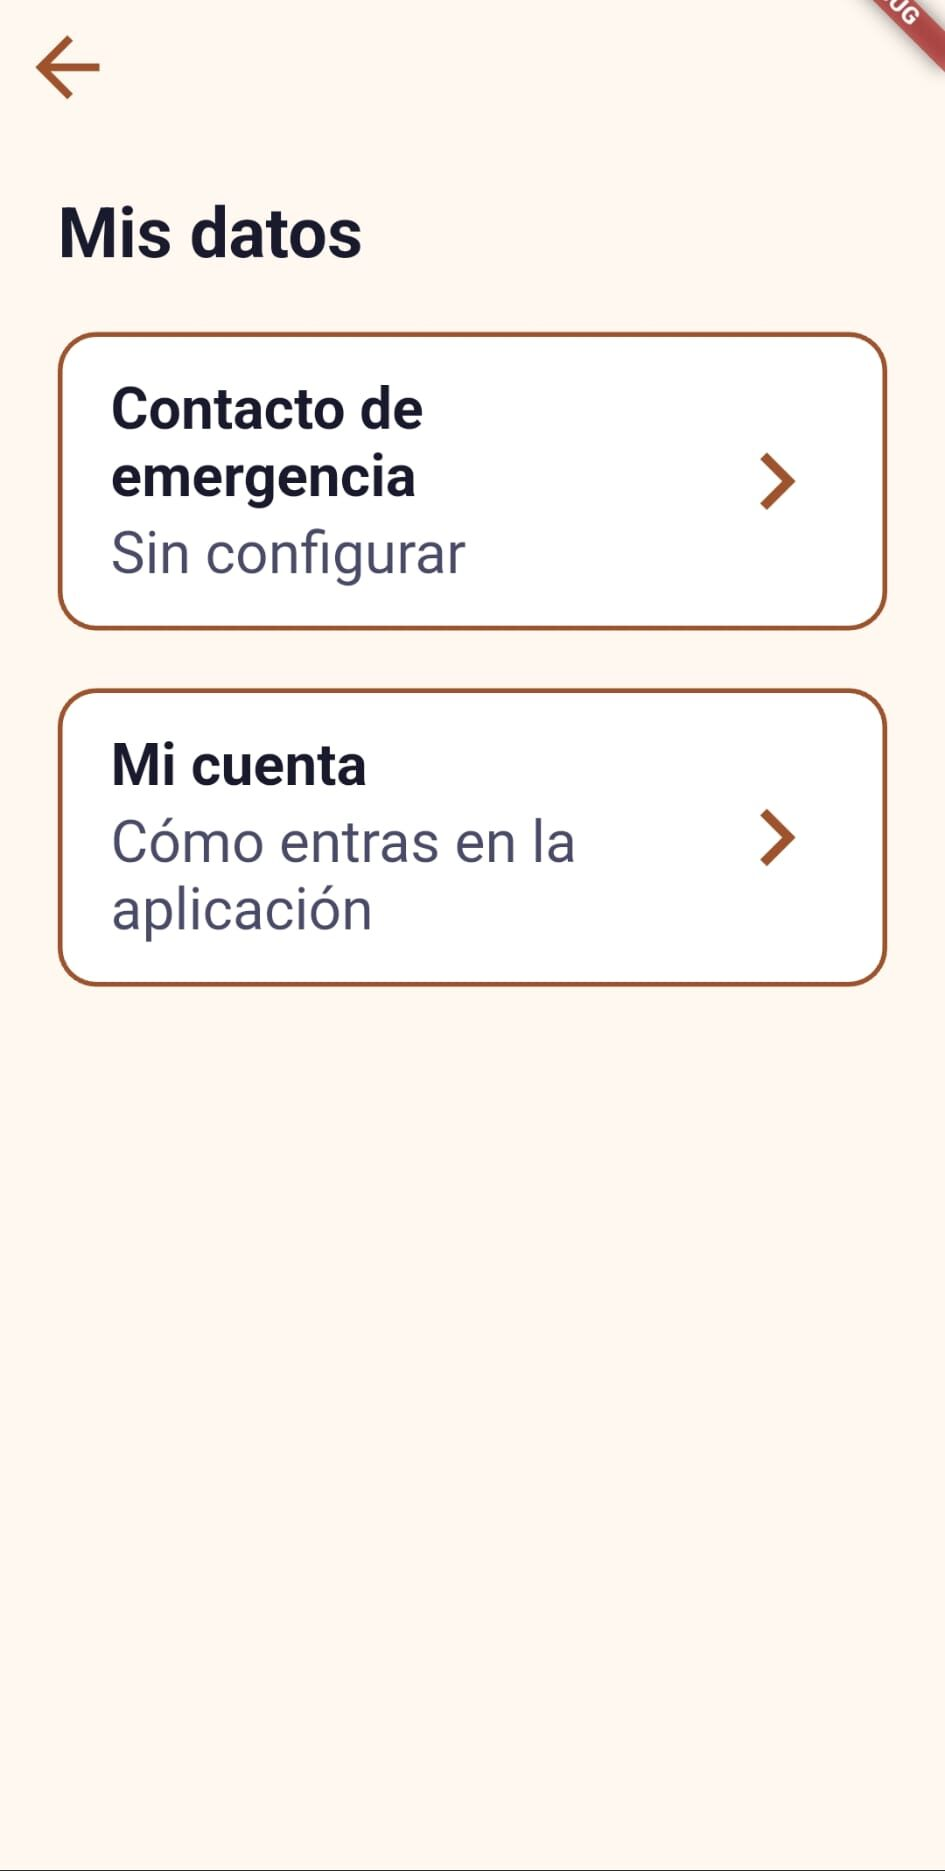
\includegraphics[width=\linewidth]{imagenes/manual/mayor-mis-datos}
    \caption{Mis datos}
  \end{subfigure}\manualhueco
  \begin{subfigure}[t]{0.165\textwidth}\centering
    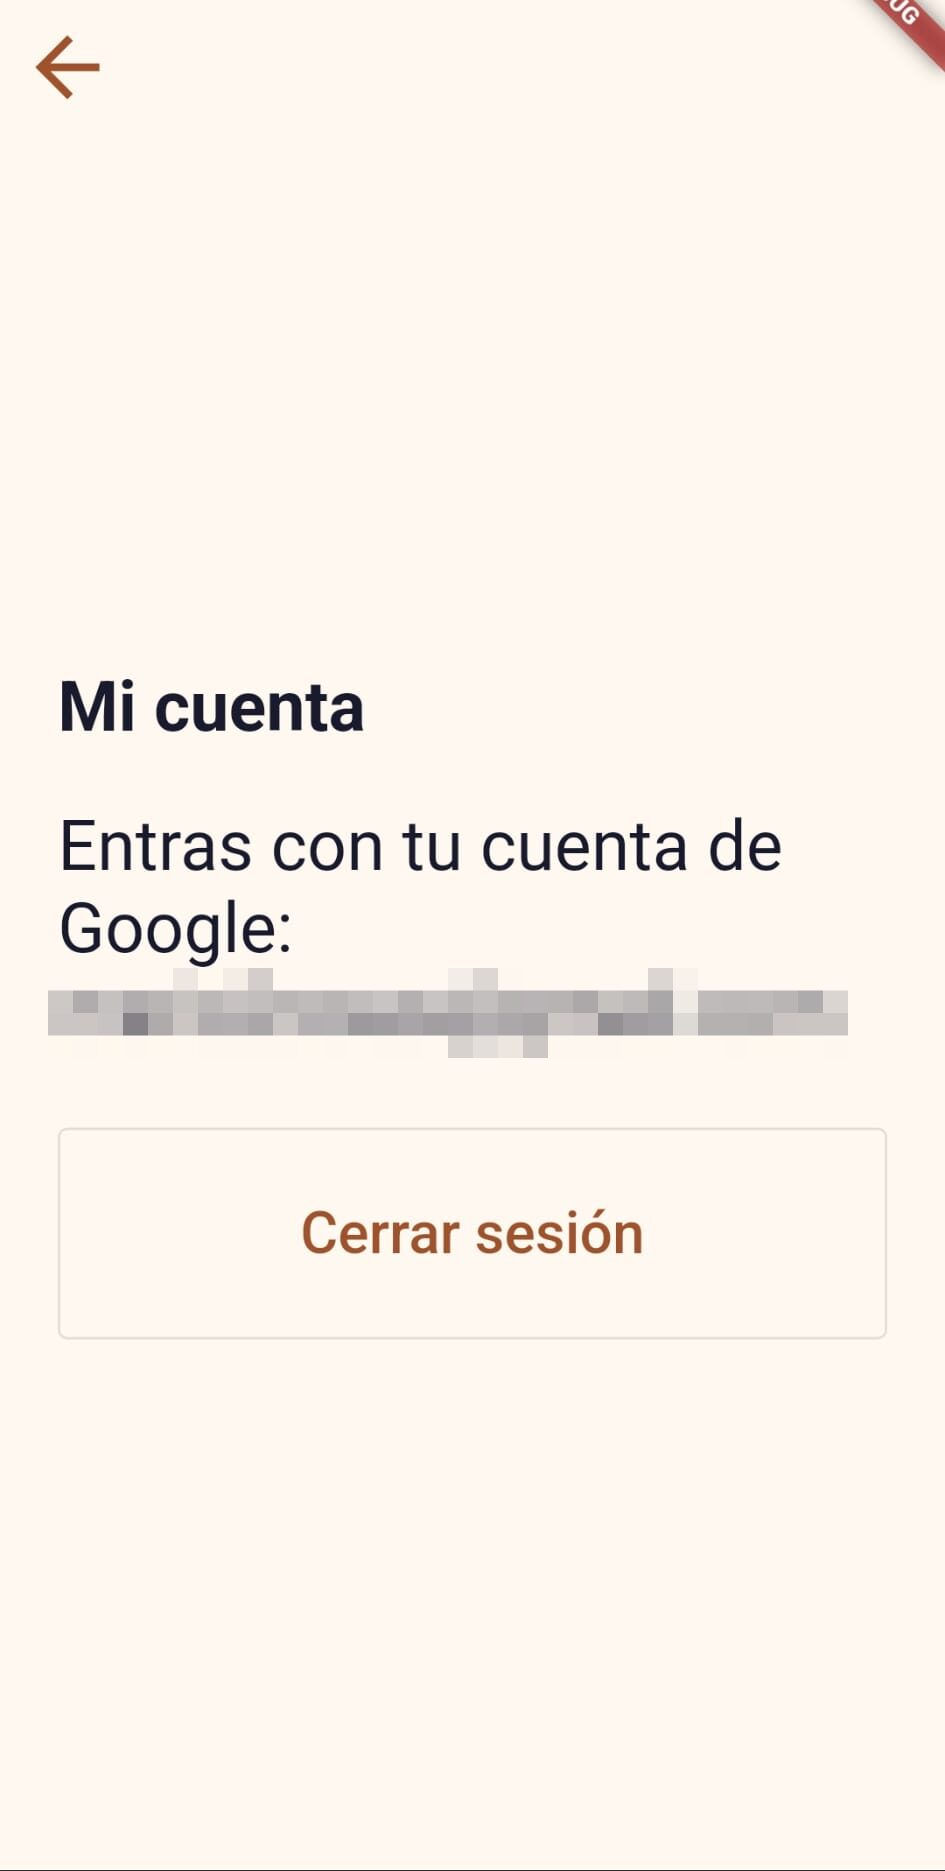
\includegraphics[width=\linewidth]{imagenes/manual/mayor-mi-cuenta}
    \caption{Mi cuenta}
  \end{subfigure}\manualhueco
  \begin{subfigure}[t]{0.165\textwidth}\centering
    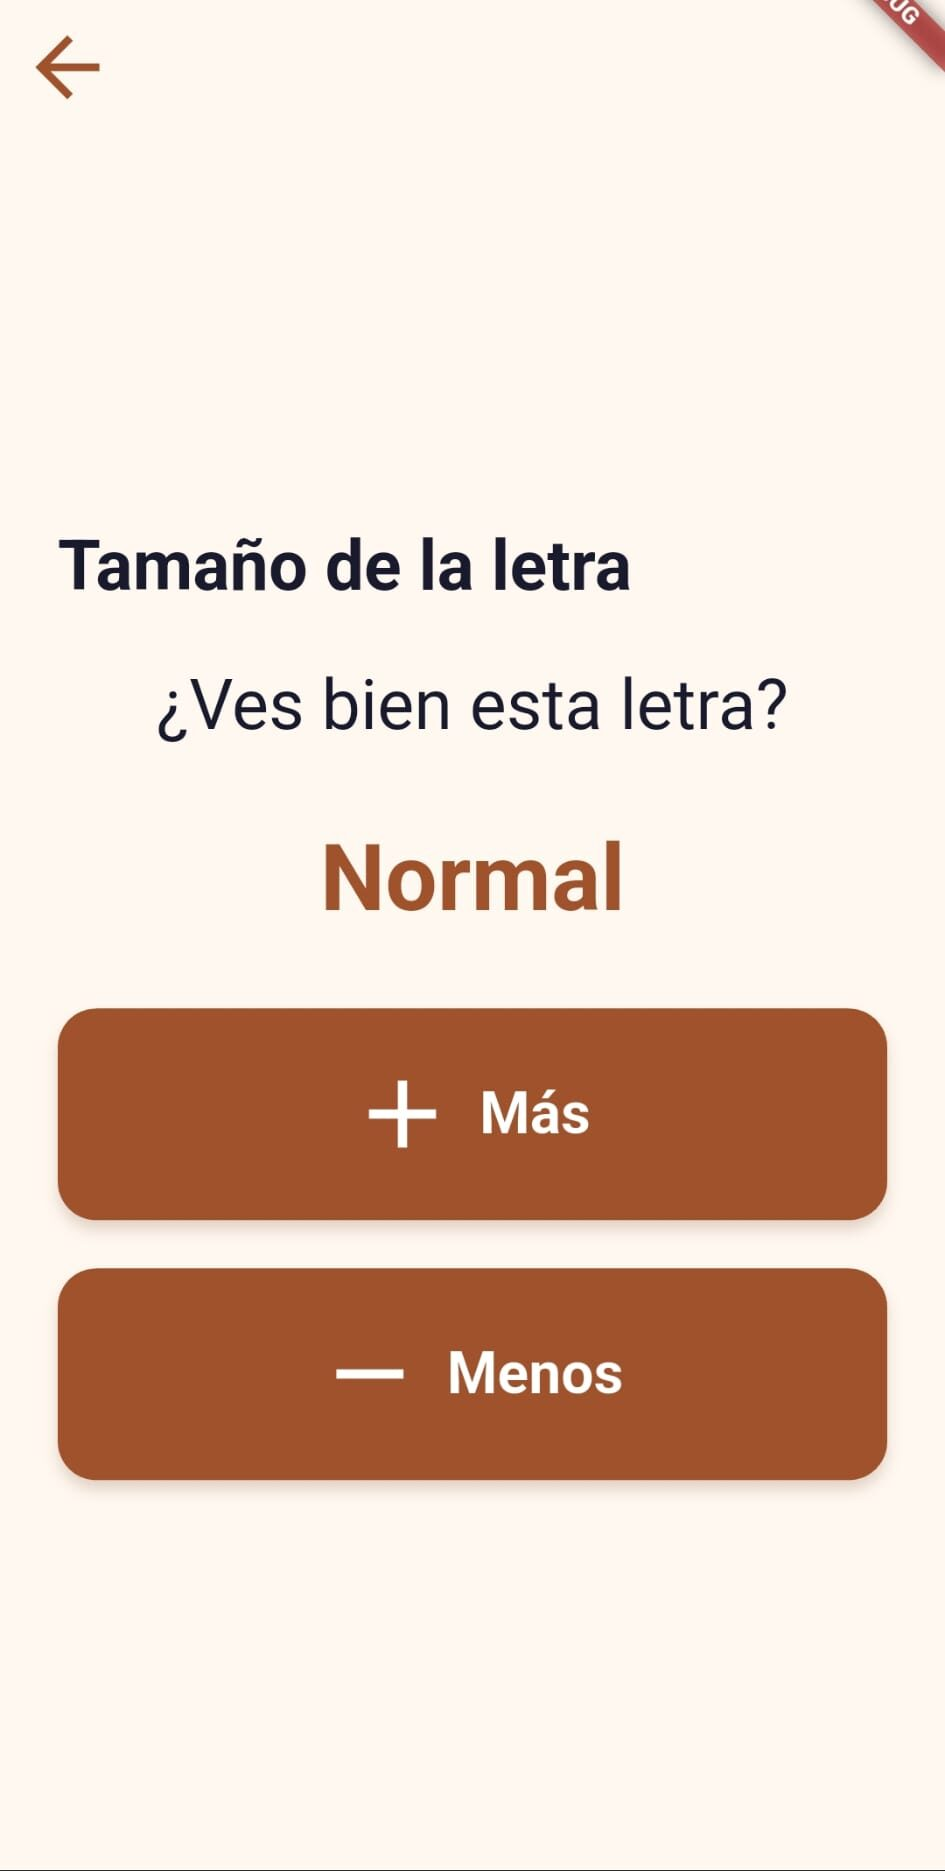
\includegraphics[width=\linewidth]{imagenes/manual/mayor-letra-normal}
    \caption{Letra normal}
  \end{subfigure}\manualhueco
  \begin{subfigure}[t]{0.165\textwidth}\centering
    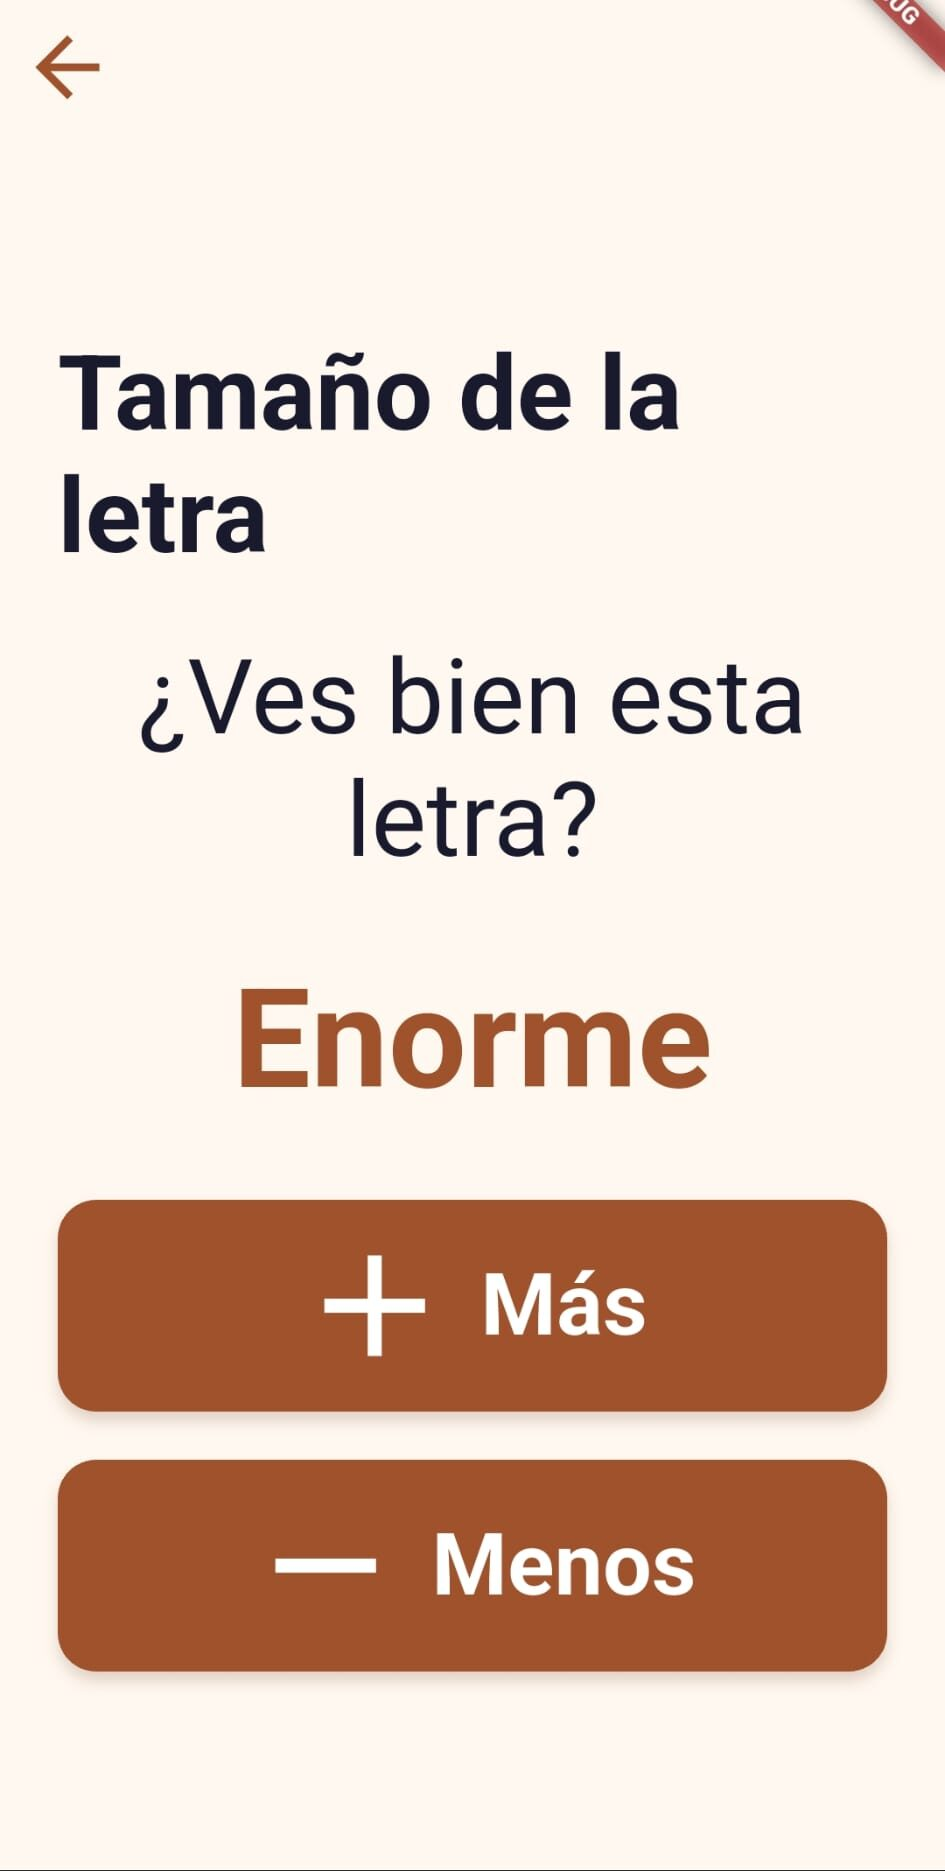
\includegraphics[width=\linewidth]{imagenes/manual/mayor-letra-enorme}
    \caption{Letra enorme}
  \end{subfigure}

  \medskip
  \begin{subfigure}[t]{0.165\textwidth}\centering
    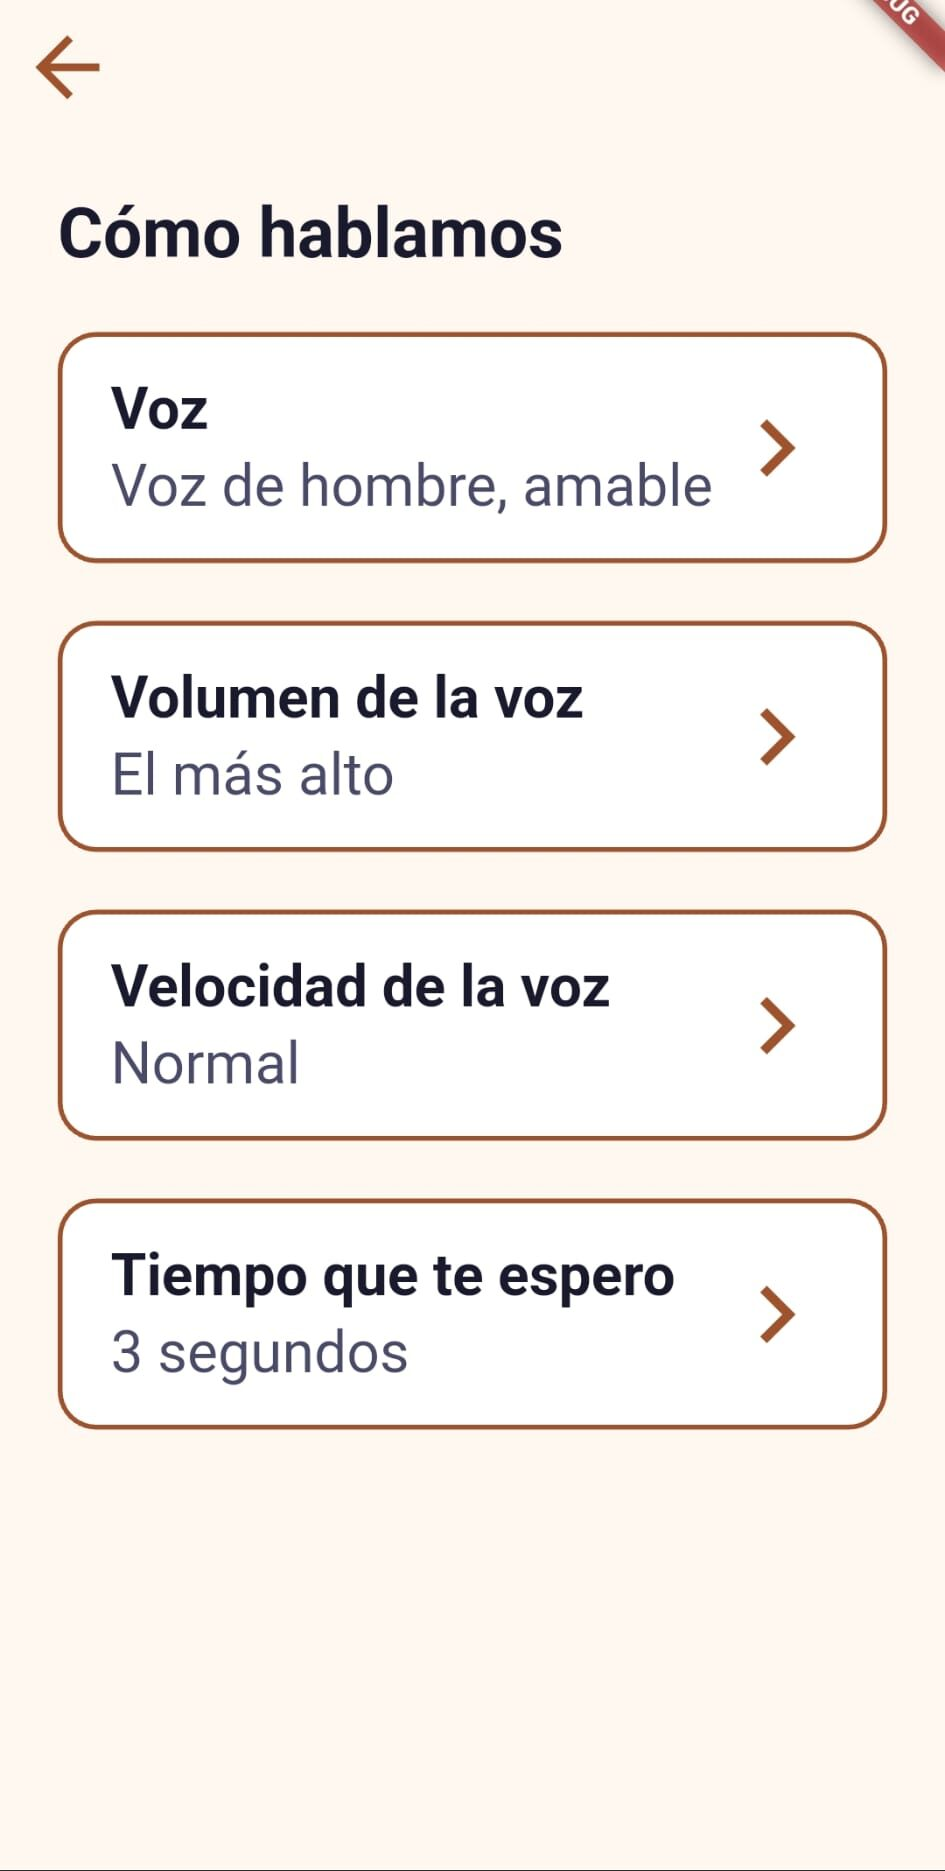
\includegraphics[width=\linewidth]{imagenes/manual/mayor-como-hablamos}
    \captionsetup{justification=centering}\caption{Cómo hablamos}
  \end{subfigure}\manualhueco
  \begin{subfigure}[t]{0.165\textwidth}\centering
    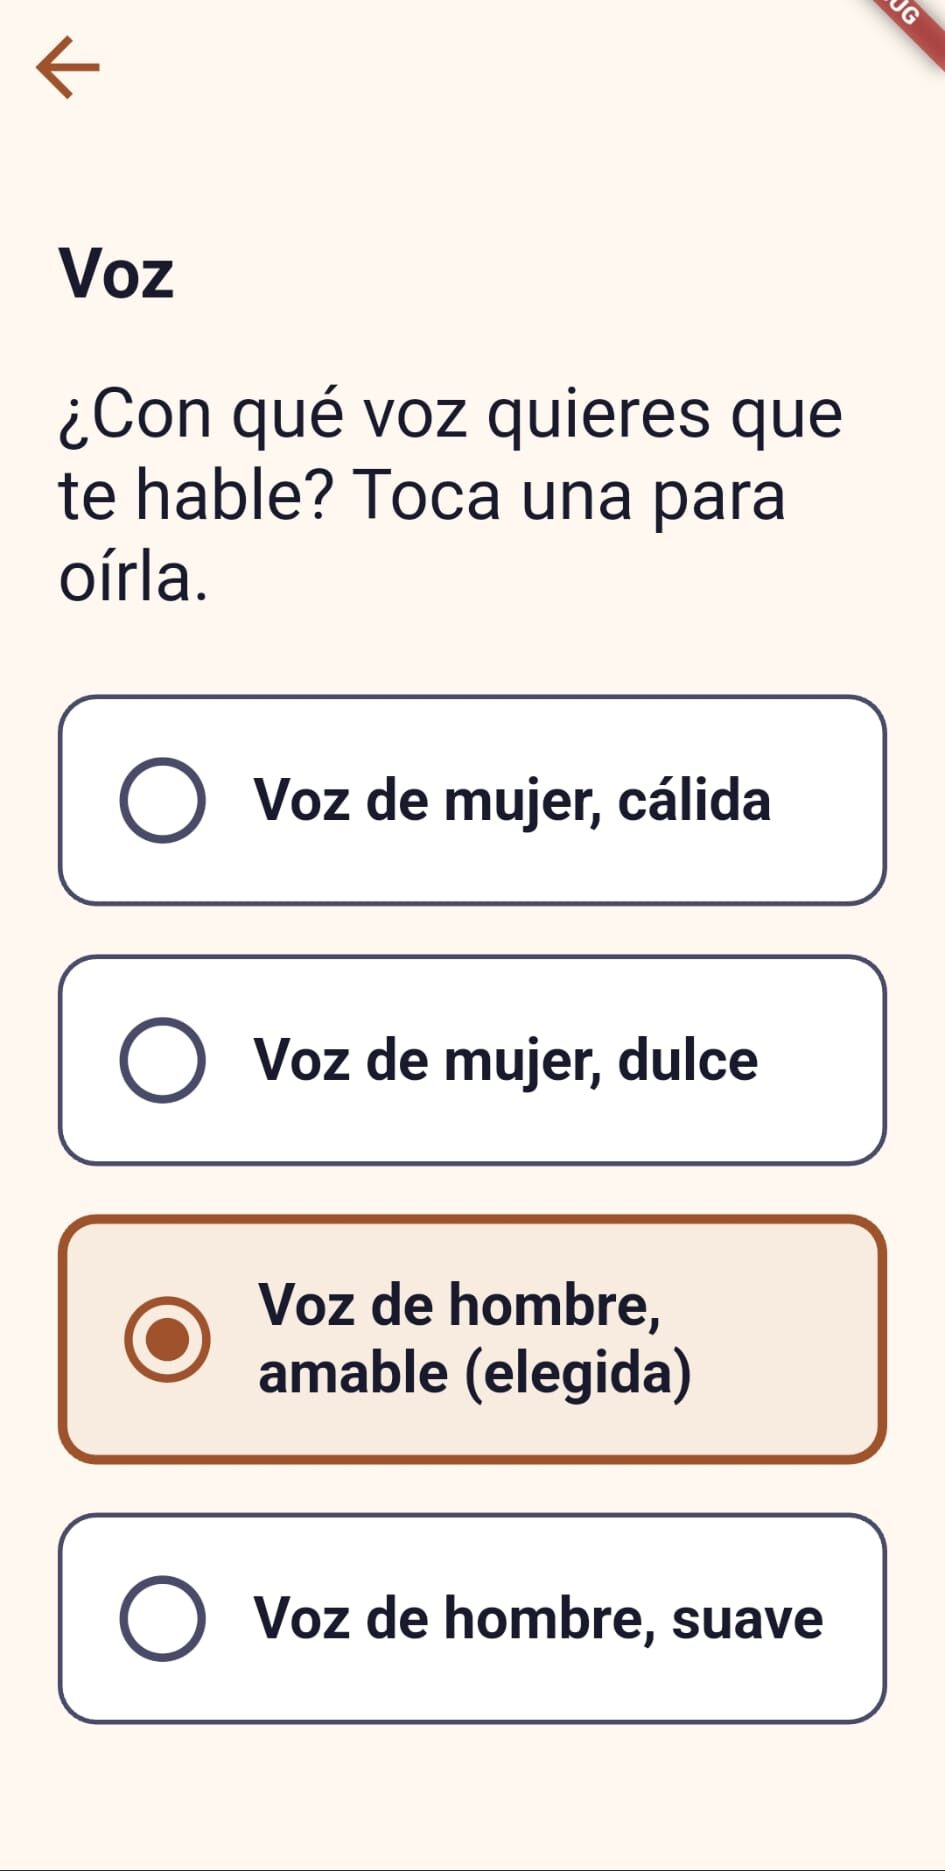
\includegraphics[width=\linewidth]{imagenes/manual/mayor-voz}
    \caption{Voz}
  \end{subfigure}\manualhueco
  \begin{subfigure}[t]{0.165\textwidth}\centering
    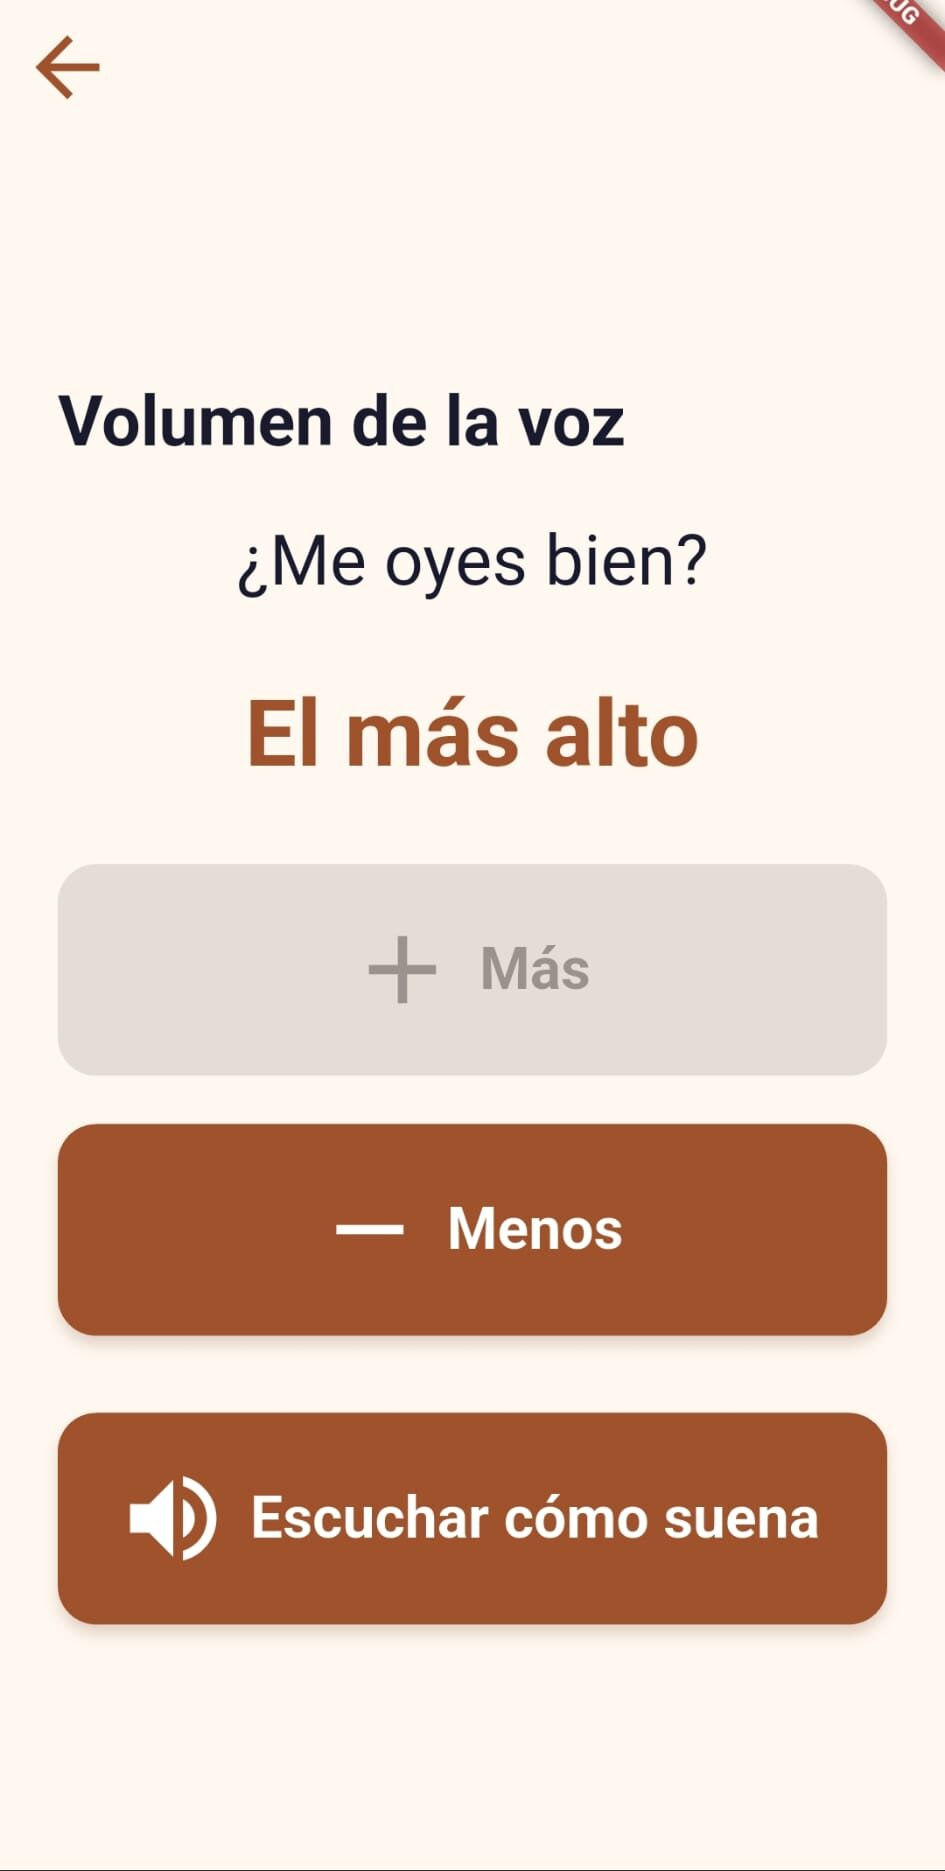
\includegraphics[width=\linewidth]{imagenes/manual/mayor-volumen}
    \caption{Volumen}
  \end{subfigure}\manualhueco
  \begin{subfigure}[t]{0.165\textwidth}\centering
    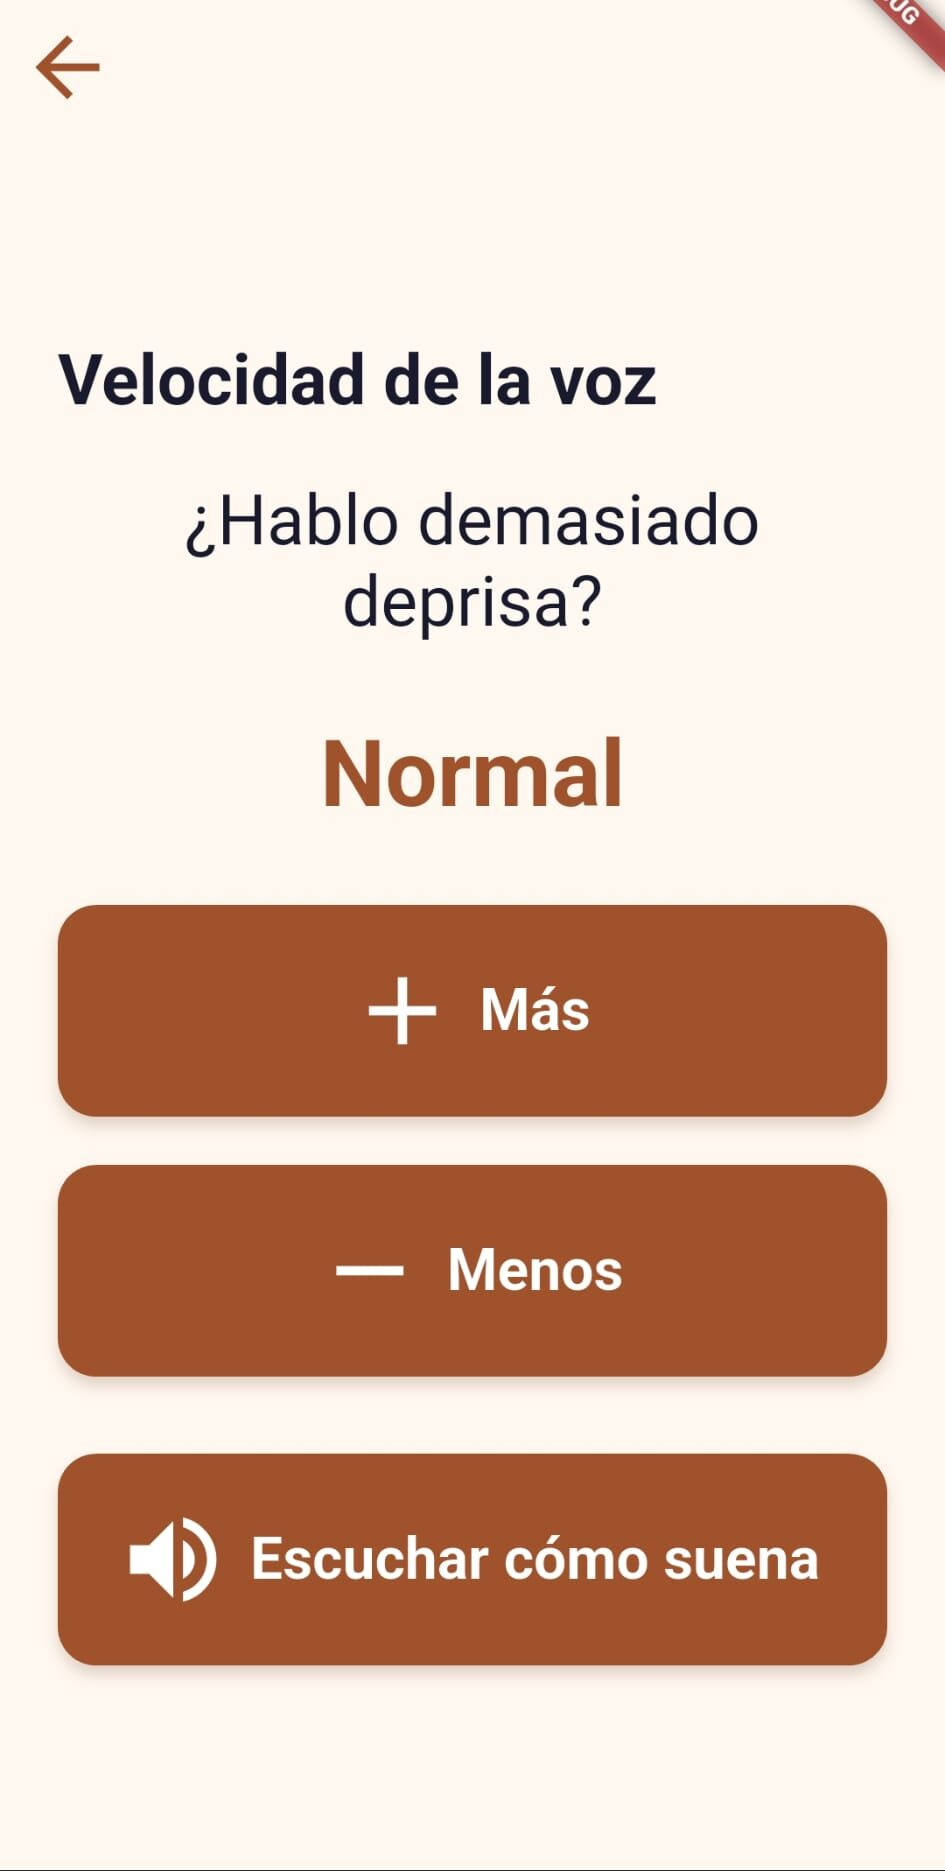
\includegraphics[width=\linewidth]{imagenes/manual/mayor-velocidad}
    \caption{Velocidad}
  \end{subfigure}\manualhueco
  \begin{subfigure}[t]{0.165\textwidth}\centering
    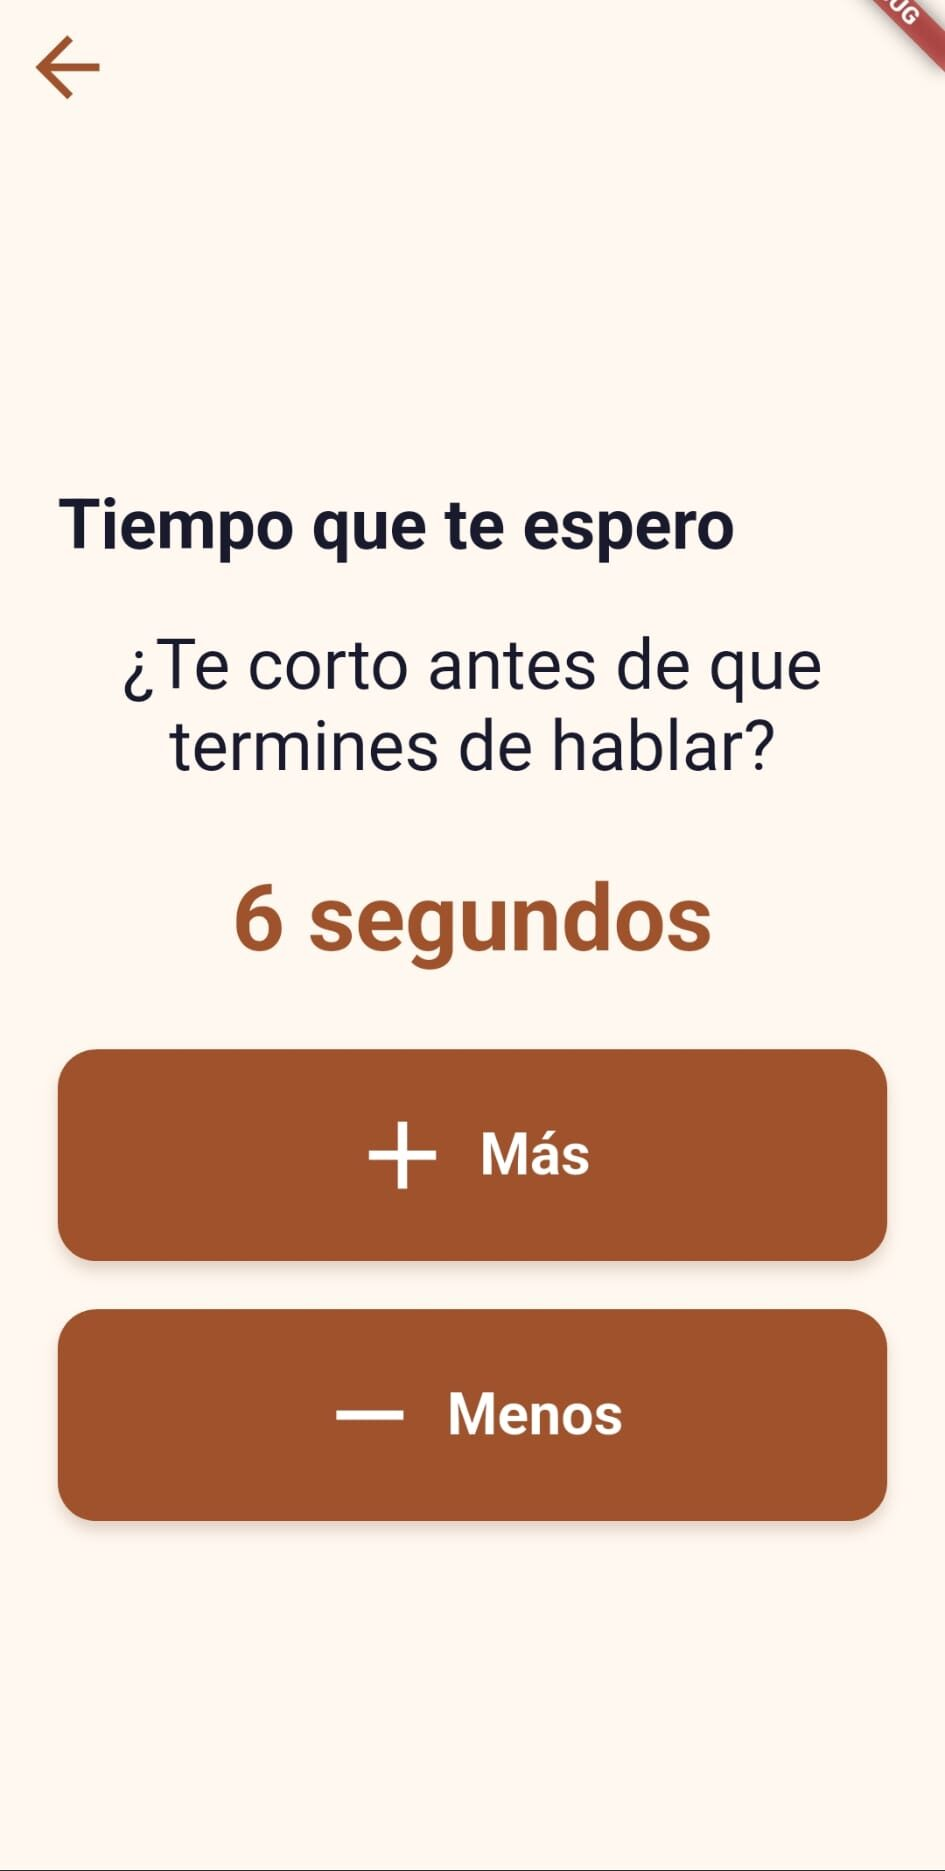
\includegraphics[width=\linewidth]{imagenes/manual/mayor-espera}
    \caption{Espera}
  \end{subfigure}
  \caption{Ajustes de la persona mayor.}
  \label{fig:manual-ajustes}
\end{figure}

La rueda de abajo a la derecha abre los ajustes, agrupados en cuatro apartados (\autoref{fig:manual-ajustes}). Todo se cambia con botones grandes, como <<Más>> y <<Menos>>, y los cambios se aplican al momento. La flecha de arriba a la izquierda vuelve a la pantalla anterior.

\begin{itemize}
  \item \textbf{Mis datos.} Su contacto de emergencia, si usa la aplicación por su cuenta, y <<Mi cuenta>>, que indica cómo entra en la aplicación. Si entró sin registrarse, desde ahí puede guardar su cuenta con Google para no perder nada al cambiar de móvil; si entra con Google, puede cerrar la sesión.
  \item \textbf{Tamaño de la letra.} La frase <<¿Ves bien esta letra?>> crece o encoge según pulse, para que compruebe con qué tamaño lee mejor.
  \item \textbf{Cómo hablamos.} La voz del asistente (al tocar una, la oye), el volumen, la velocidad y el tiempo que espera en silencio antes de contestar. El volumen y la velocidad se prueban con <<Escuchar cómo suena>>.
  \item \textbf{Mis conversaciones.} Qué se guarda de lo que hablan, como se explica a continuación.
\end{itemize}

\subsection{Mis conversaciones y <<Mi semana>>}
\label{sec:manual-mi-semana}

En <<Mis conversaciones>> decide qué se guarda de lo que habla con el asistente (\autoref{fig:manual-conversaciones}):

\begin{figure}[!htb]\centering
  \begin{subfigure}[t]{0.165\textwidth}\centering
    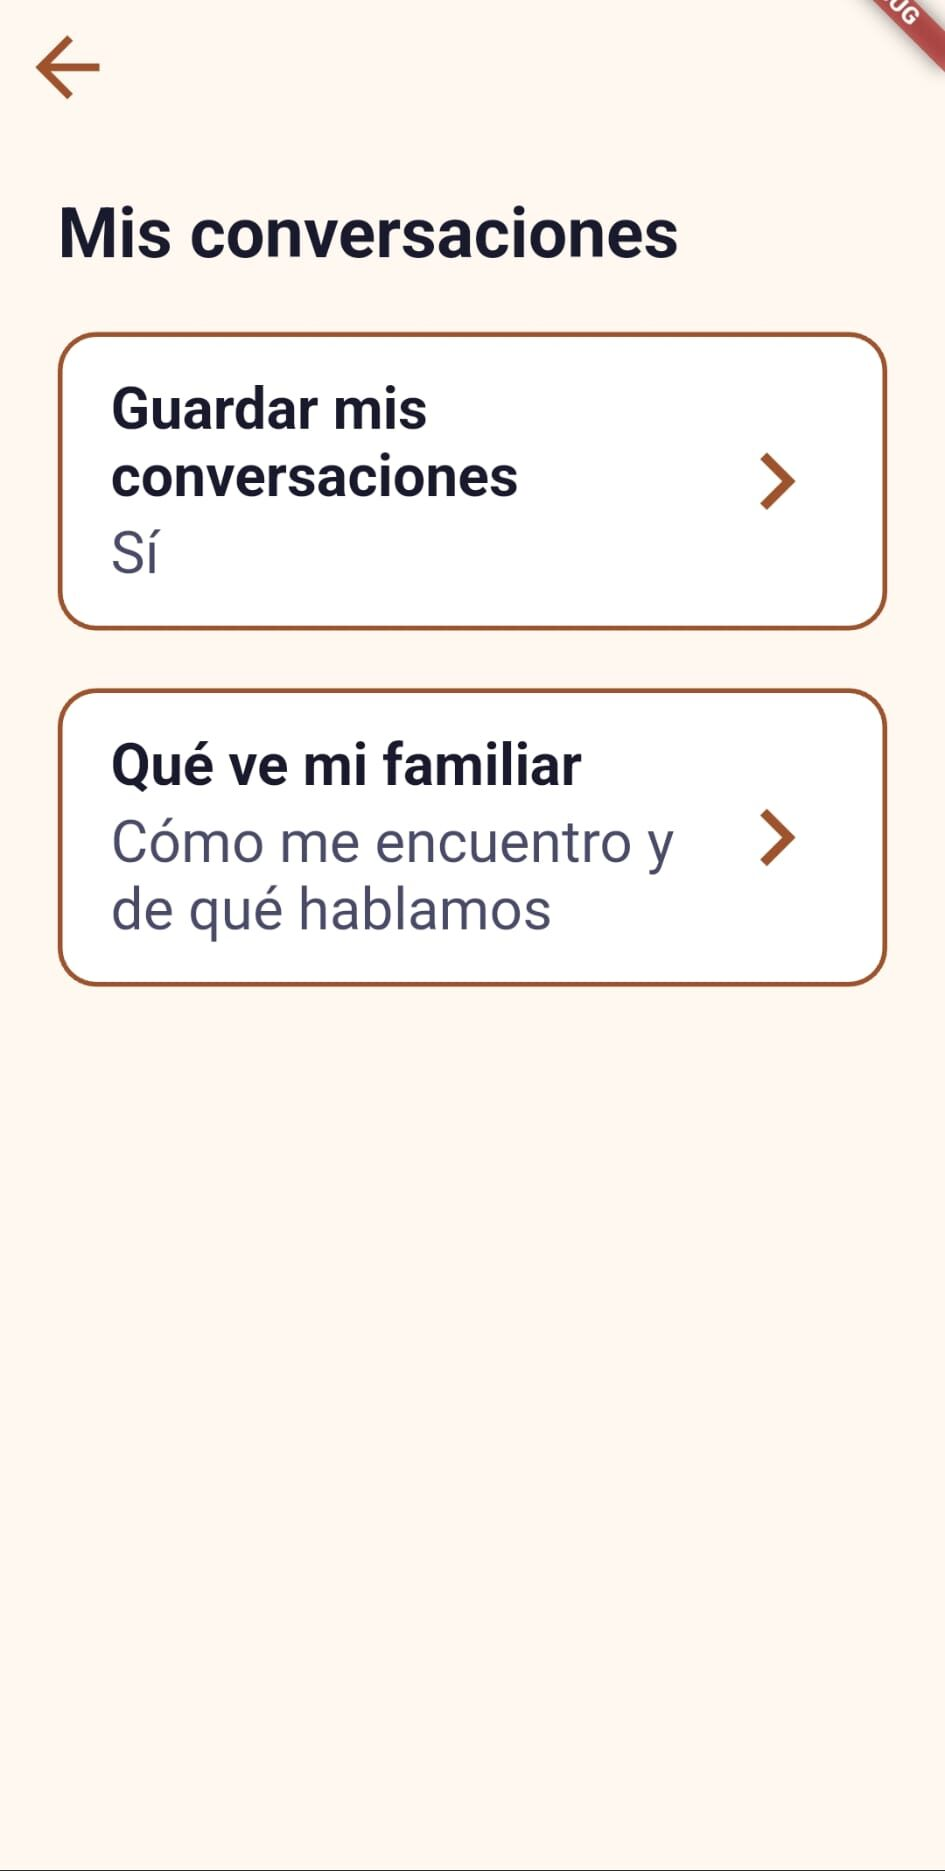
\includegraphics[width=\linewidth]{imagenes/manual/mayor-conversaciones}
    \caption{Opciones}
  \end{subfigure}\manualhueco
  \begin{subfigure}[t]{0.165\textwidth}\centering
    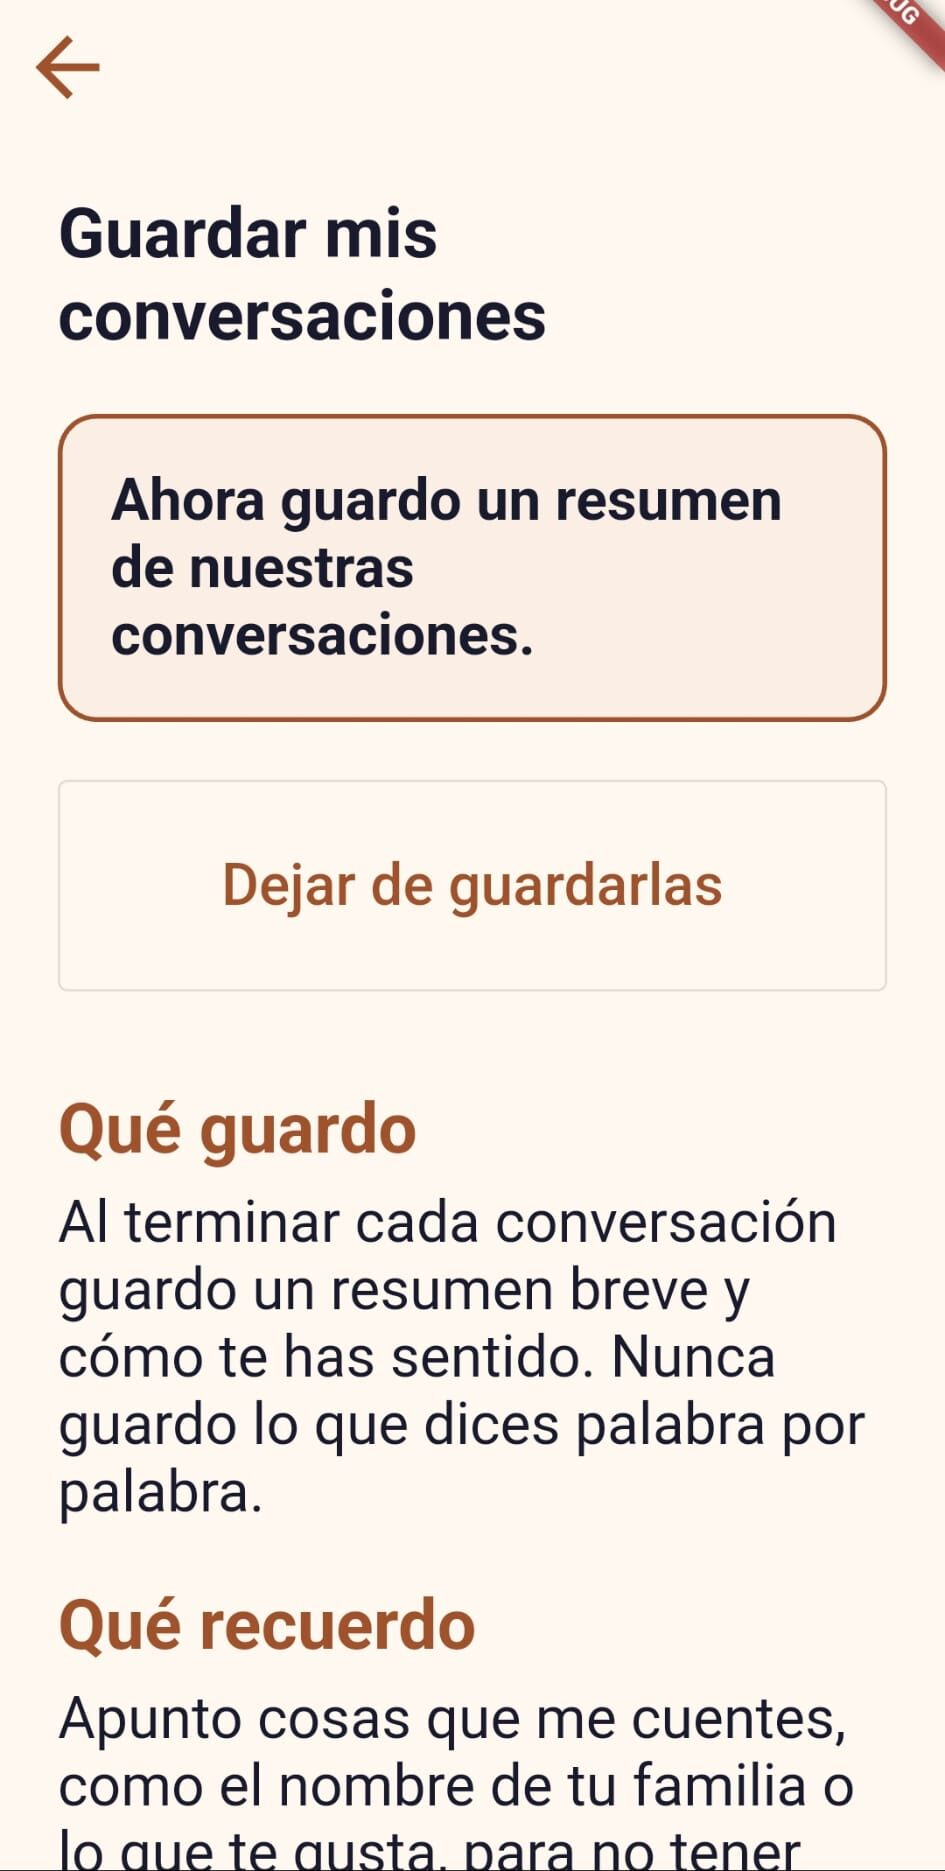
\includegraphics[width=\linewidth]{imagenes/manual/mayor-guardar}
    \caption{Guardar}
  \end{subfigure}\manualhueco
  \begin{subfigure}[t]{0.165\textwidth}\centering
    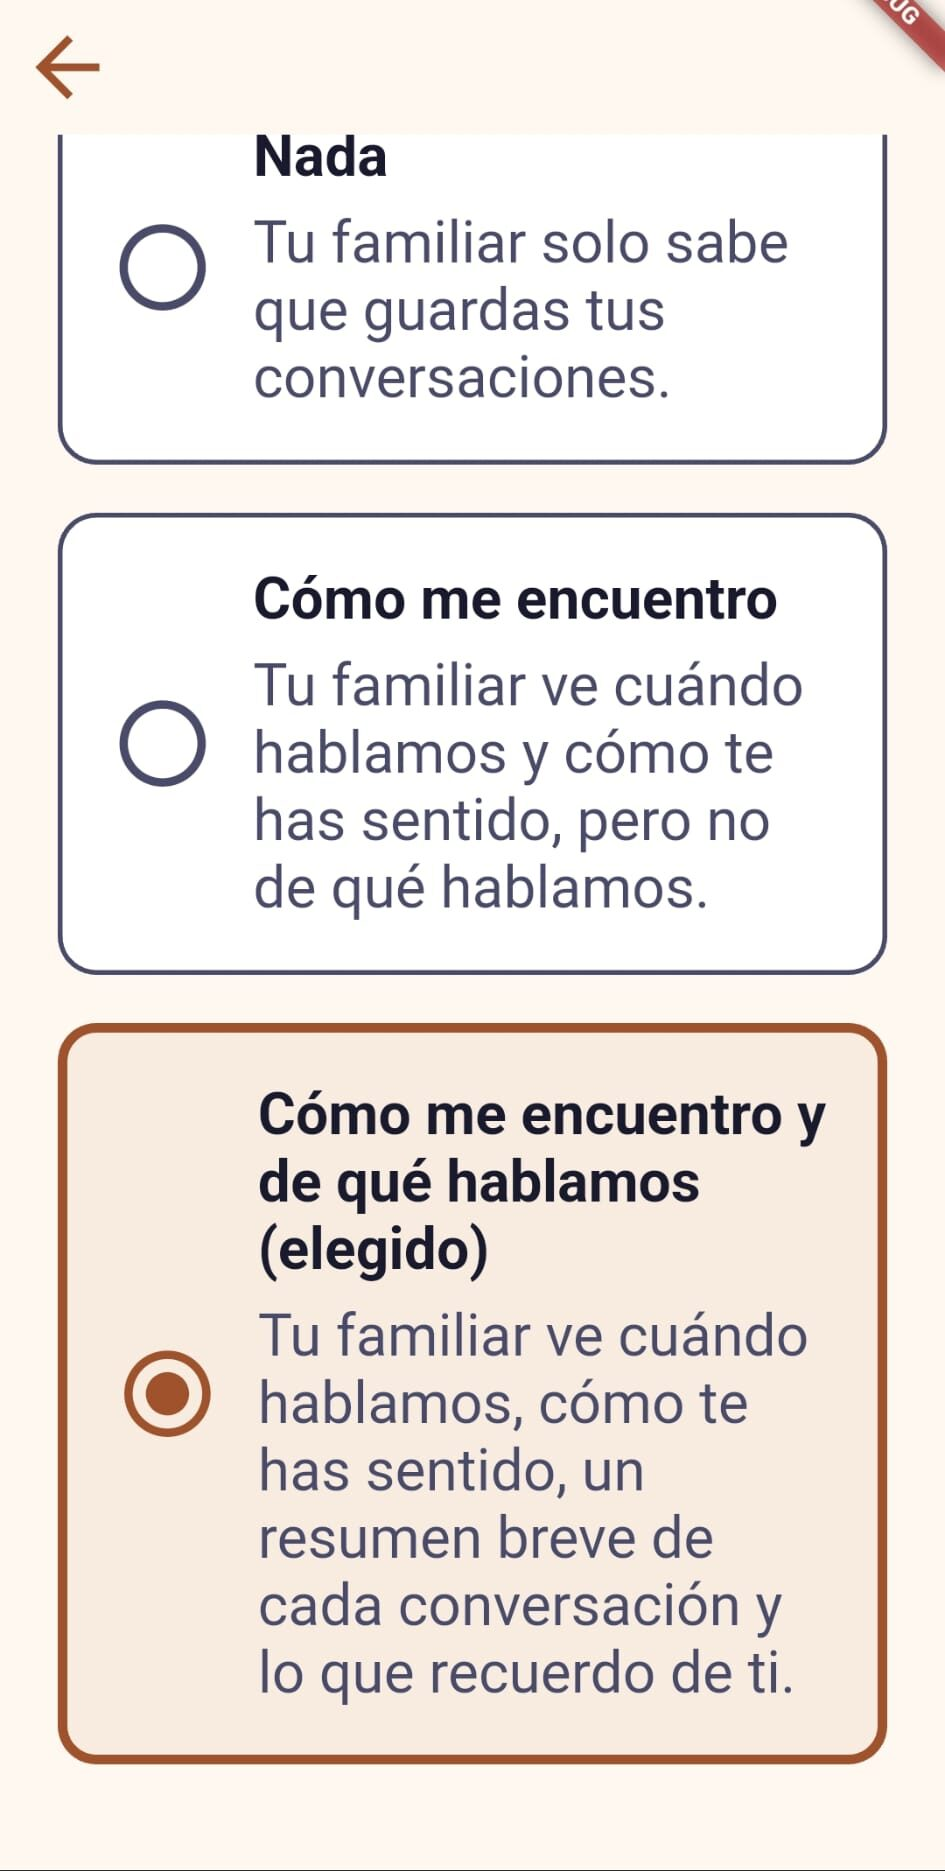
\includegraphics[width=\linewidth]{imagenes/manual/mayor-que-ve-familiar}
    \caption{Qué comparte}
  \end{subfigure}\manualhueco
  \begin{subfigure}[t]{0.165\textwidth}\centering
    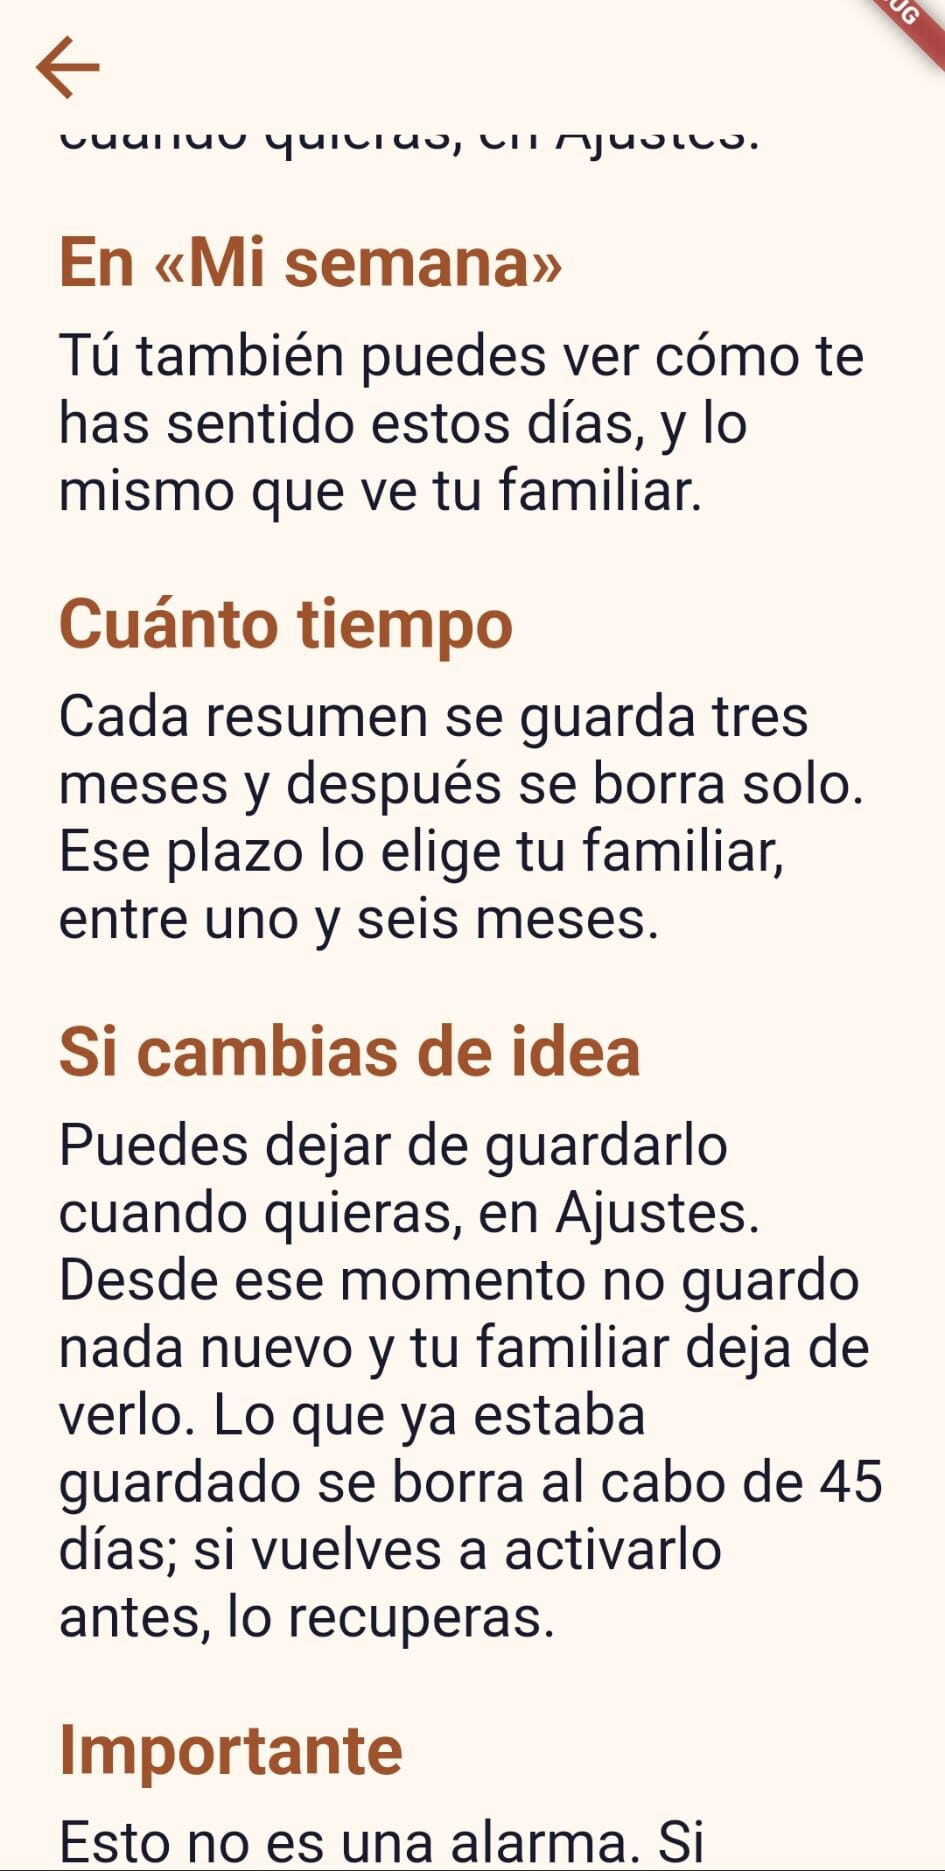
\includegraphics[width=\linewidth]{imagenes/manual/mayor-saber-mas}
    \caption{Saber más}
  \end{subfigure}\manualhueco
  \begin{subfigure}[t]{0.165\textwidth}\centering
    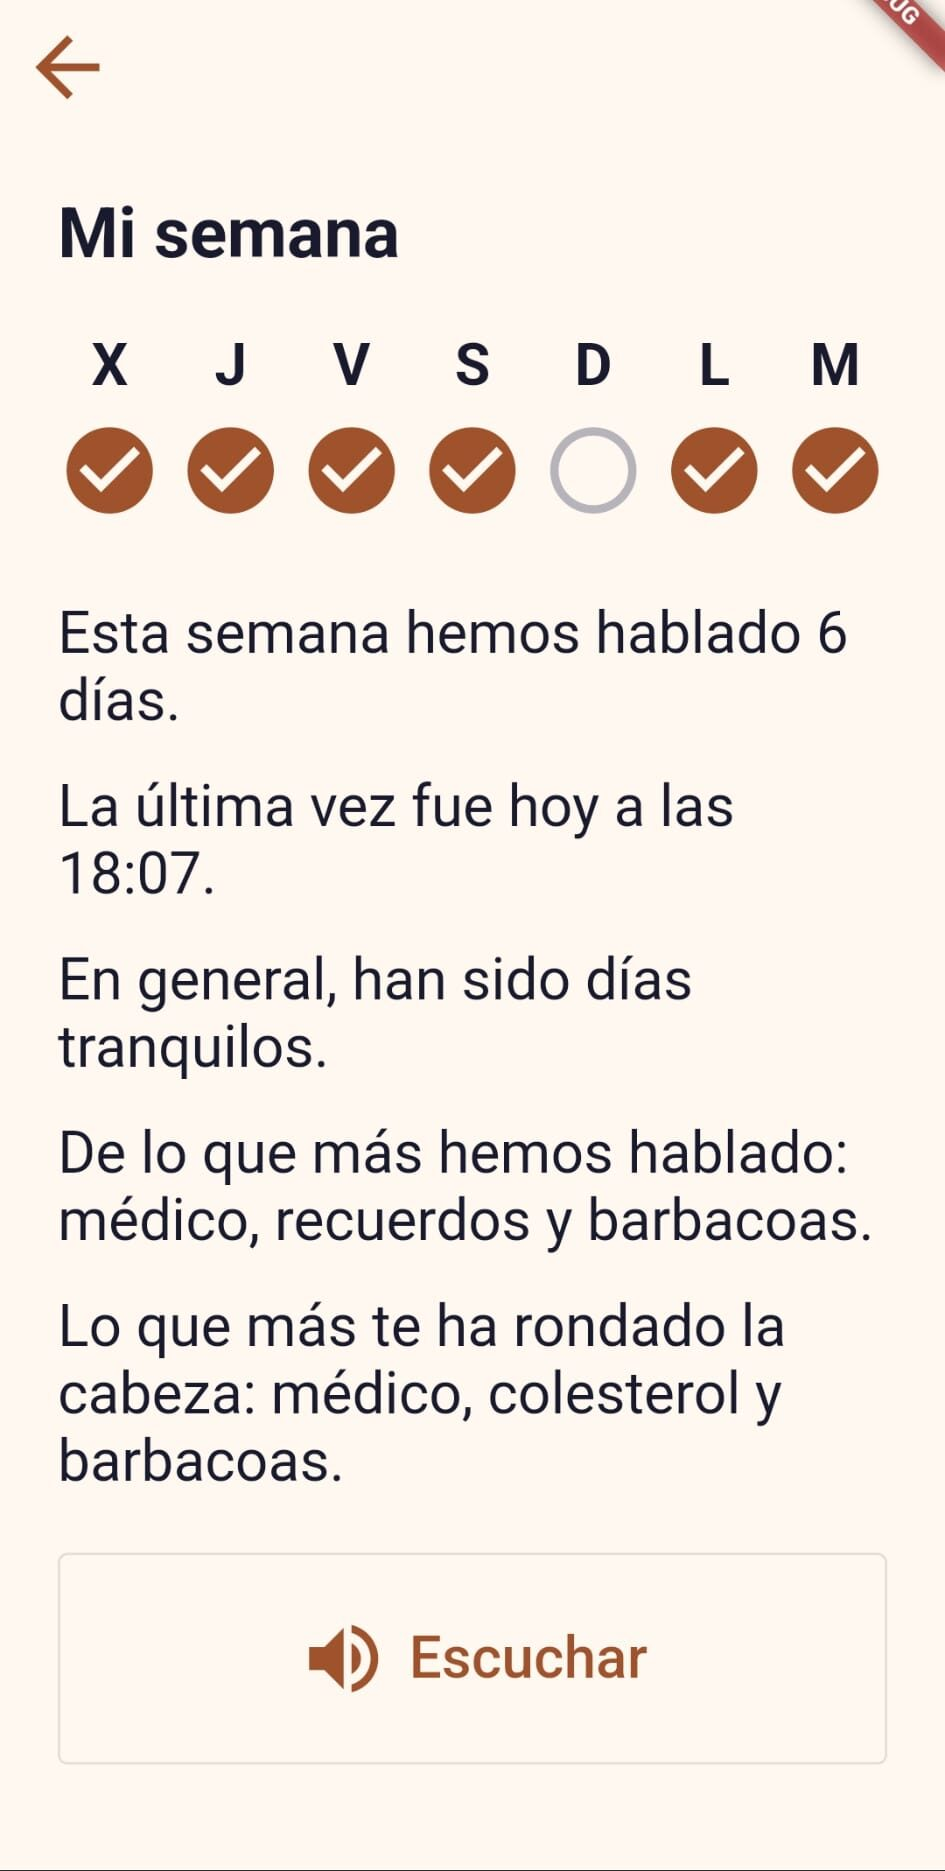
\includegraphics[width=\linewidth]{imagenes/manual/mayor-mi-semana}
    \caption{Mi semana}
  \end{subfigure}
  \caption{Lo que se guarda de las conversaciones y <<Mi semana>>.}
  \label{fig:manual-conversaciones}
\end{figure}

\begin{itemize}
  \item \textbf{Guardar mis conversaciones.} Activa o detiene el resumen. Si deja de guardarlas, desde ese momento no se guarda nada nuevo y su familiar deja de verlo. Lo que ya estaba guardado se borra pasado un tiempo, y la pantalla le indica la fecha; si vuelve a activarlo antes, lo recupera.
  \item \textbf{Qué ve mi familiar}, si está vinculado: nada (solo sabrá que guarda sus conversaciones), cómo se encuentra, o cómo se encuentra y de qué hablan. Lo elige usted y puede cambiarlo cuando quiera.
  \item \textbf{Cuándo termina una conversación} y \textbf{cuánto tiempo se guardan}, si usa la aplicación por su cuenta. Si está vinculado, estos plazos los elige su familiar.
\end{itemize}

<<Mi semana>>, en la pantalla principal, le cuenta con frases sencillas cómo ha ido su semana: qué días han conversado, cómo le ha notado el asistente, de qué han hablado más y lo que más le ha rondado la cabeza. <<Escuchar>> se lo lee en voz alta. Al final indica qué ve su familiar, con un botón para cambiarlo.

\section{El familiar}
\label{sec:manual-familiar}

\subsection{Crear la cuenta y vincularse}

En la primera pantalla de la aplicación, toque <<Soy el acompañante>> y después <<Crear una cuenta nueva>>, o <<Ya tengo una cuenta>> si ya se registró. El registro pide su nombre, un correo electrónico, una contraseña de al menos seis caracteres y su teléfono, que es el número al que llamará la persona mayor desde su botón de emergencia. Después escriba el código de cuatro caracteres que aparece en el móvil de la persona mayor cuando elige <<Vincular con mi familiar>> y pulse <<Vincular>> (\autoref{fig:manual-familiar}). Hecho esto, se abre el panel de control.

\begin{figure}[!htb]\centering
  \begin{subfigure}[t]{0.165\textwidth}\centering
    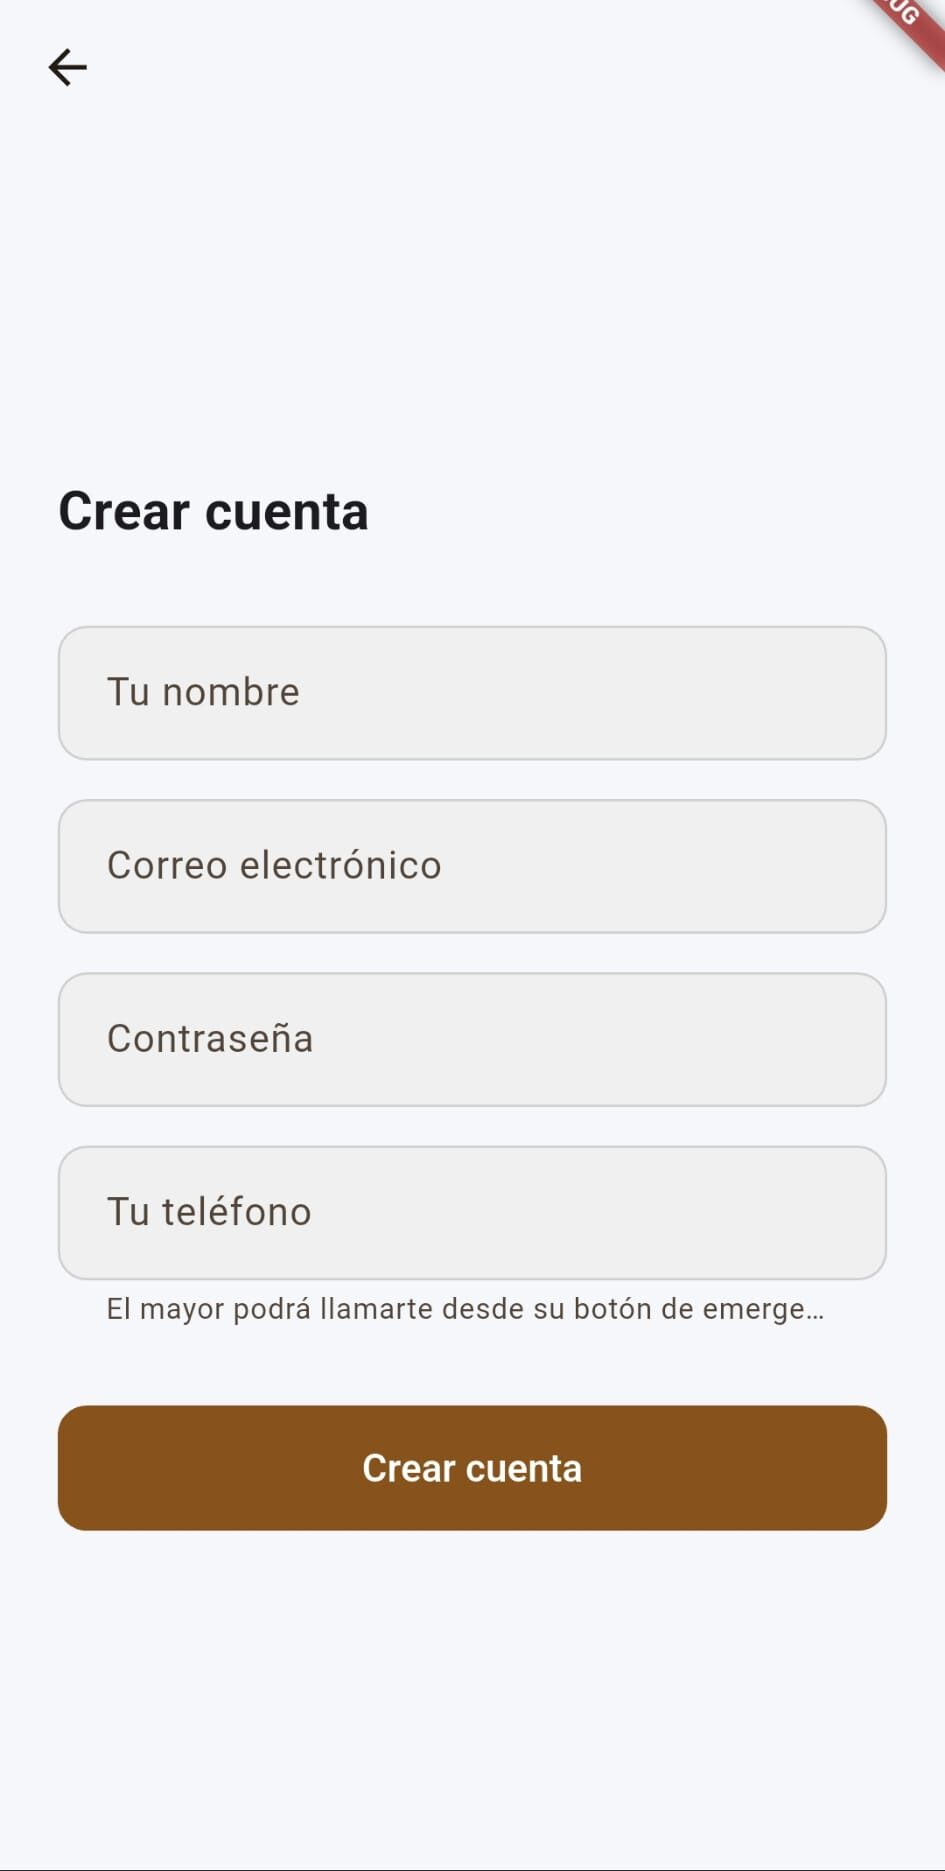
\includegraphics[width=\linewidth]{imagenes/manual/familiar-registro}
    \caption{Registro}
  \end{subfigure}\manualhueco
  \begin{subfigure}[t]{0.165\textwidth}\centering
    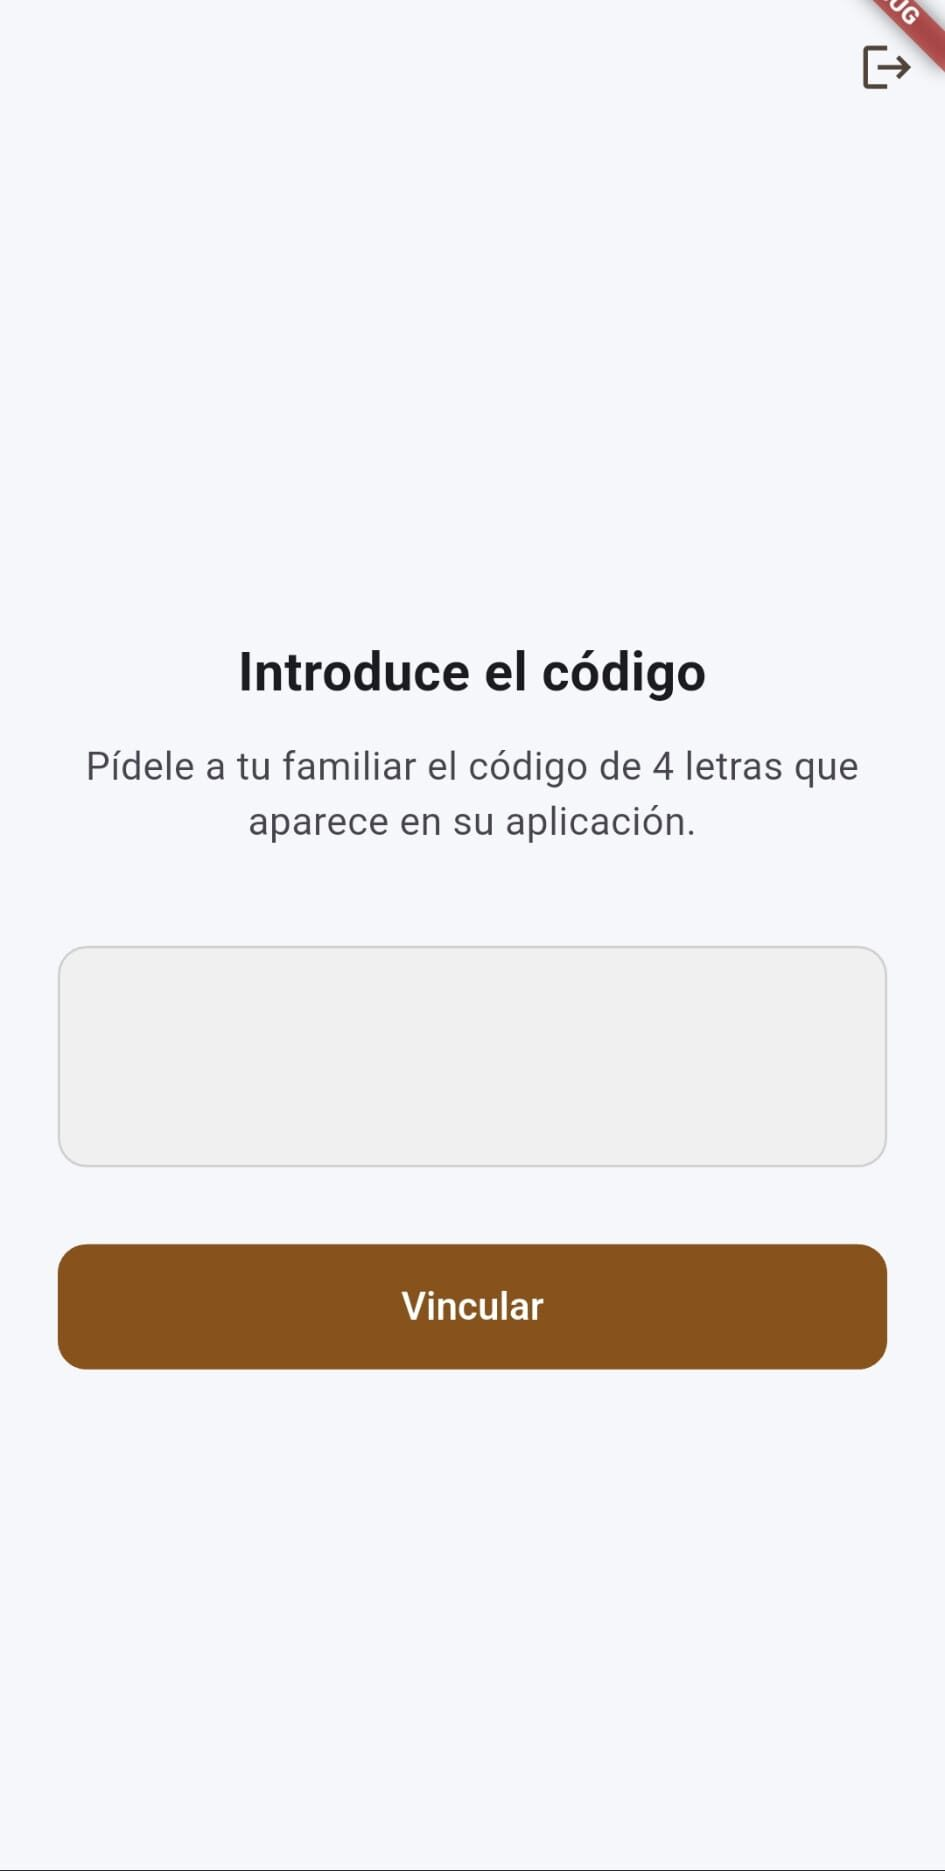
\includegraphics[width=\linewidth]{imagenes/manual/familiar-codigo}
    \caption{Código}
  \end{subfigure}\manualhueco
  \begin{subfigure}[t]{0.165\textwidth}\centering
    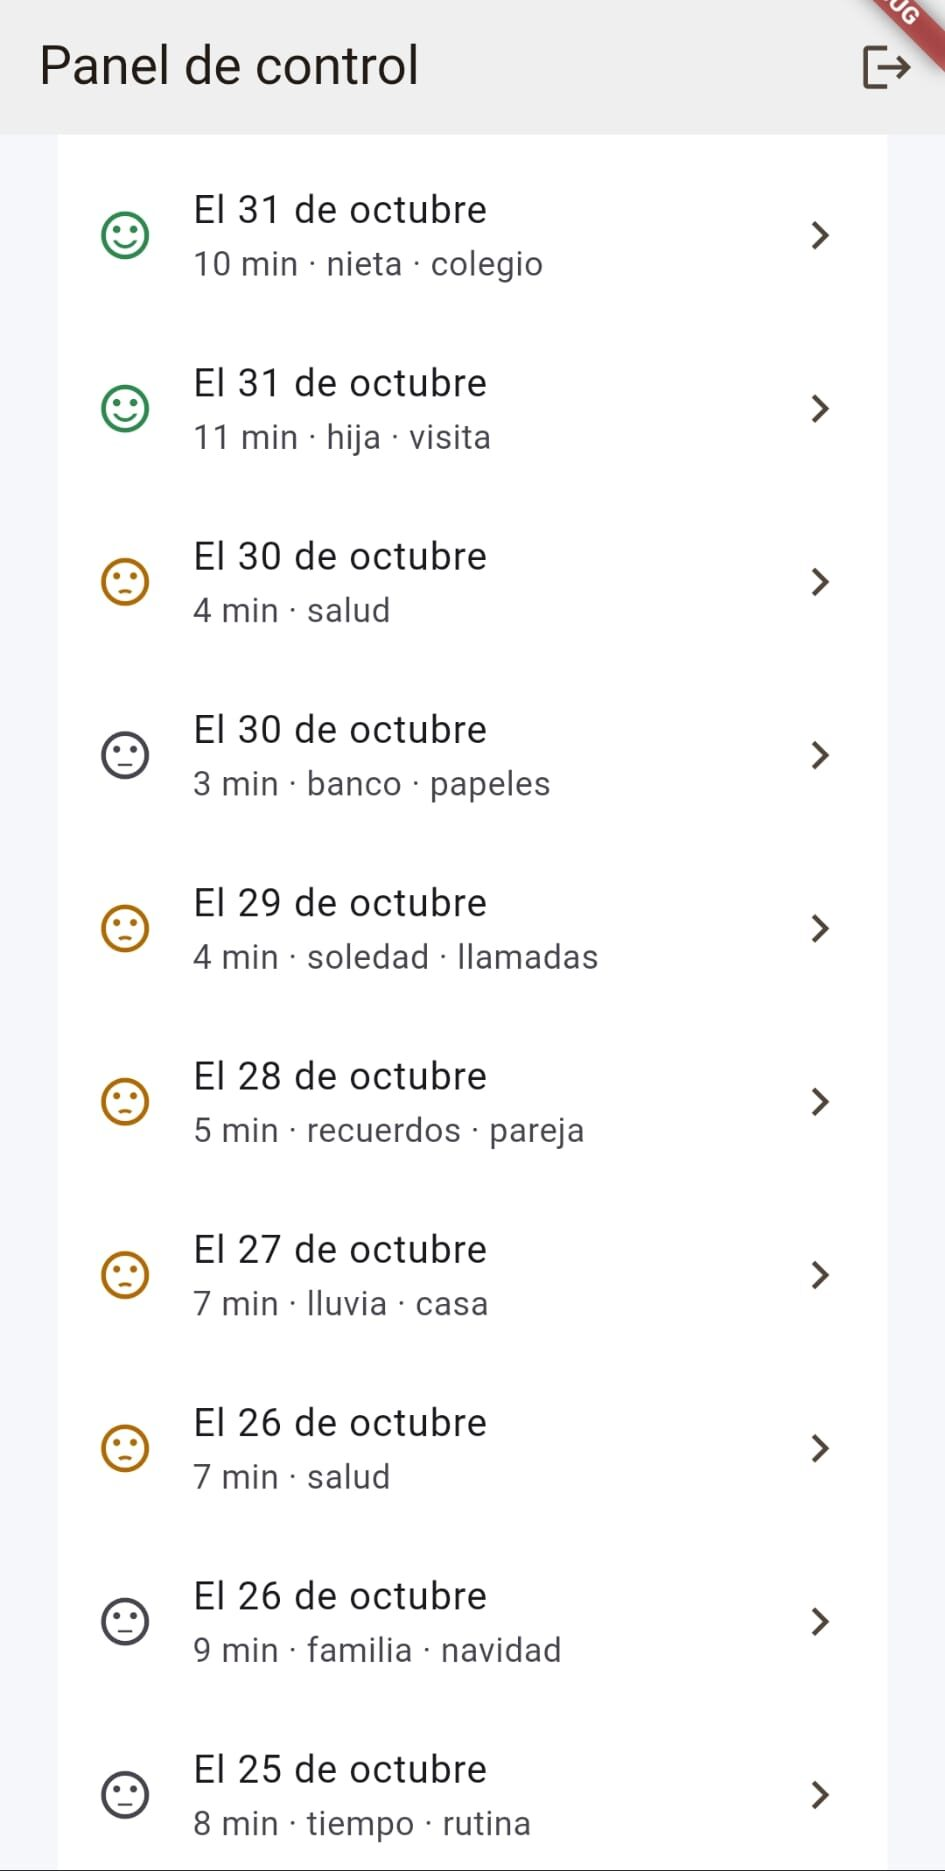
\includegraphics[width=\linewidth]{imagenes/manual/familiar-conversaciones}
    \caption{Lista}
  \end{subfigure}\manualhueco
  \begin{subfigure}[t]{0.165\textwidth}\centering
    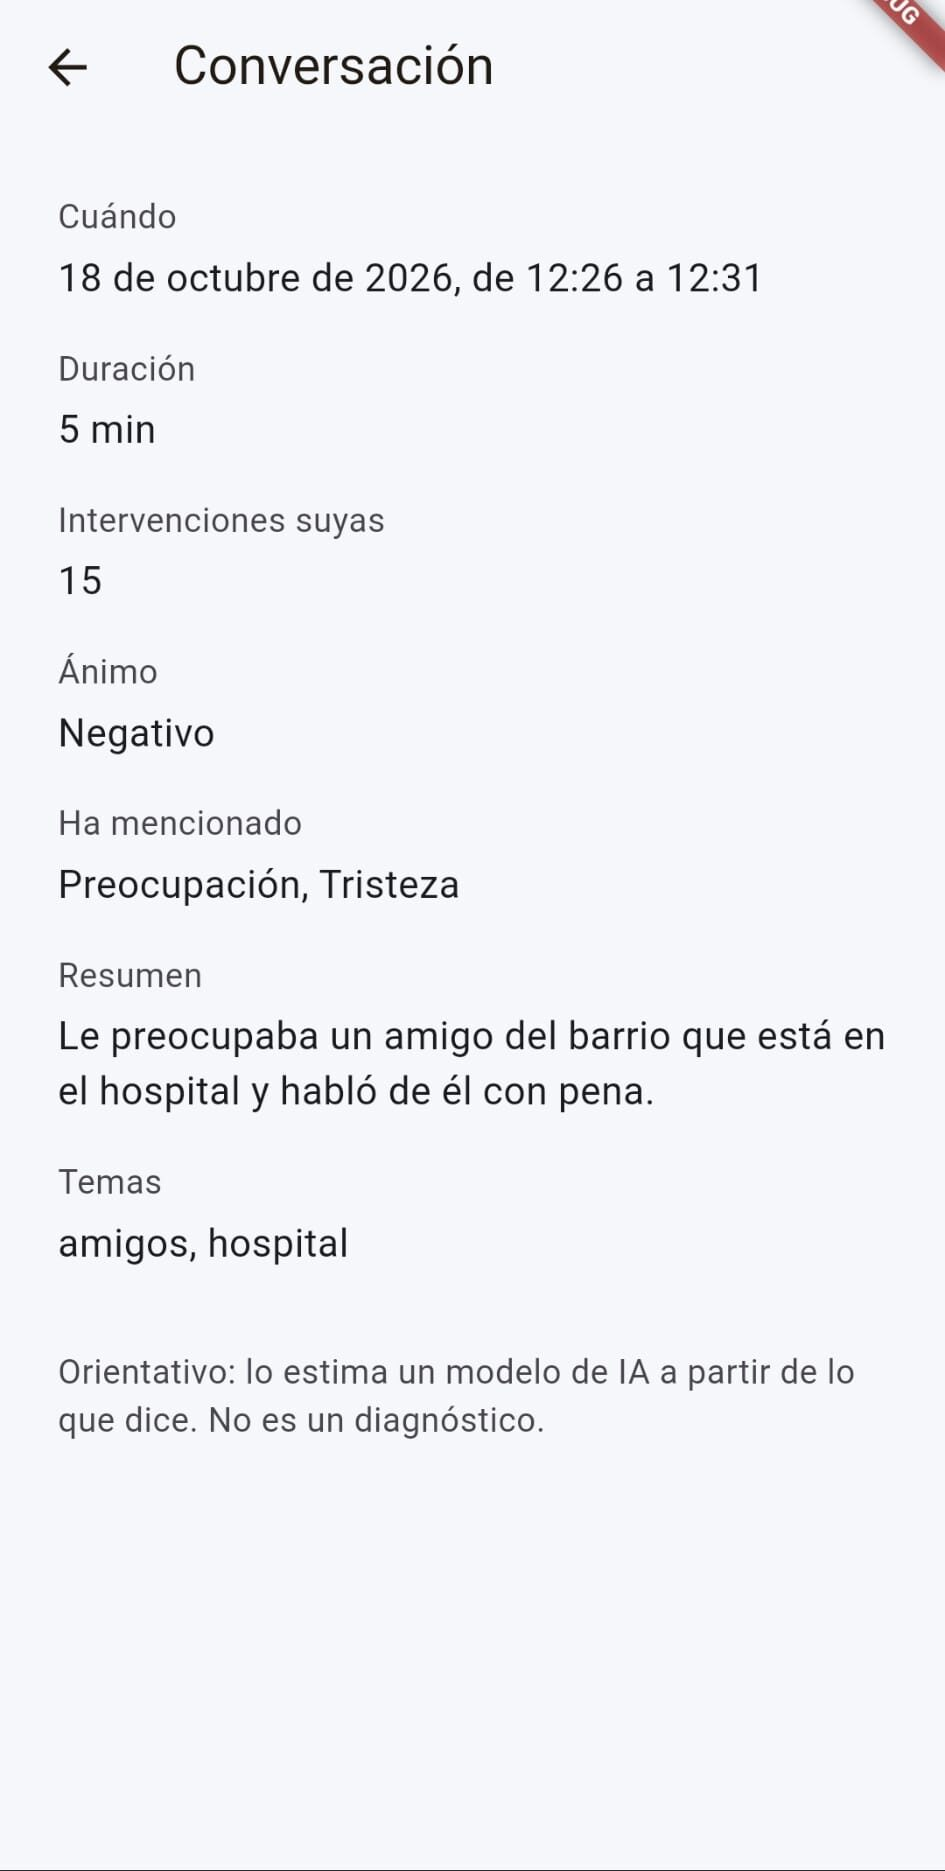
\includegraphics[width=\linewidth]{imagenes/manual/familiar-detalle}
    \caption{Detalle}
  \end{subfigure}\manualhueco
  \begin{subfigure}[t]{0.165\textwidth}\centering
    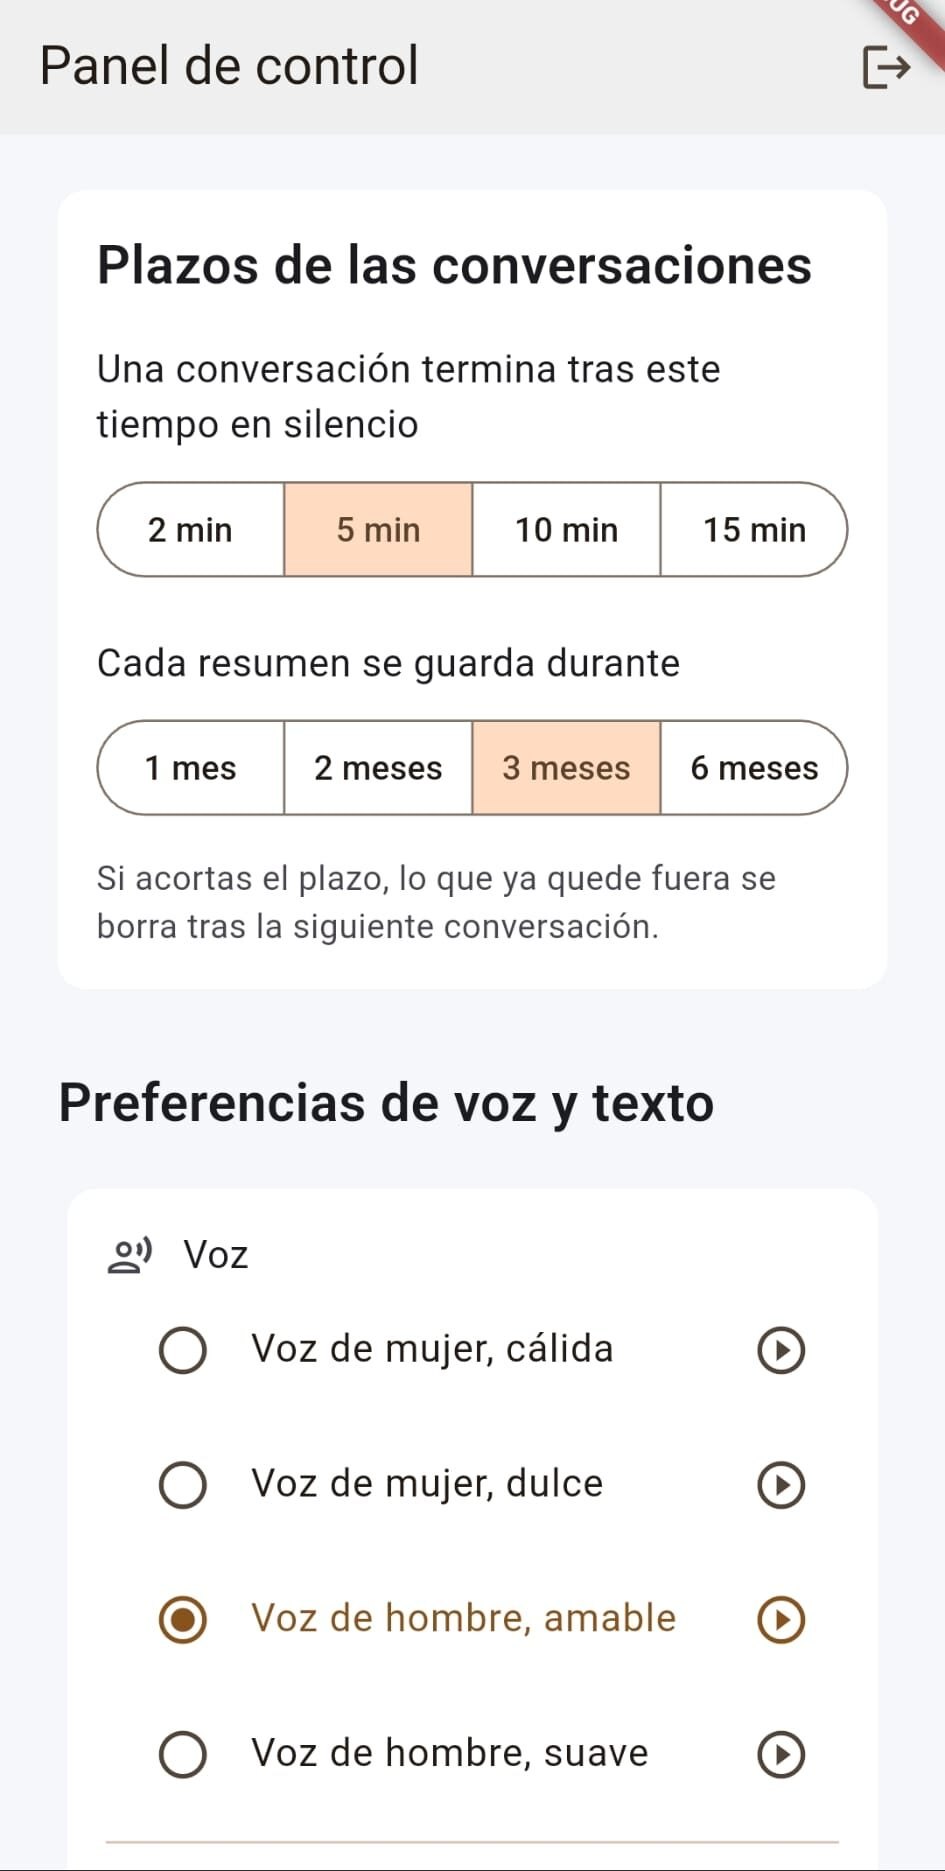
\includegraphics[width=\linewidth]{imagenes/manual/familiar-plazos}
    \caption{Plazos}
  \end{subfigure}
  \caption{Alta del familiar y otras pantallas del panel.}
  \label{fig:manual-familiar}
\end{figure}

\subsection{El panel de control}

\begin{figure}[!htb]\centering
  \begin{subfigure}[t]{0.27\textwidth}\centering
    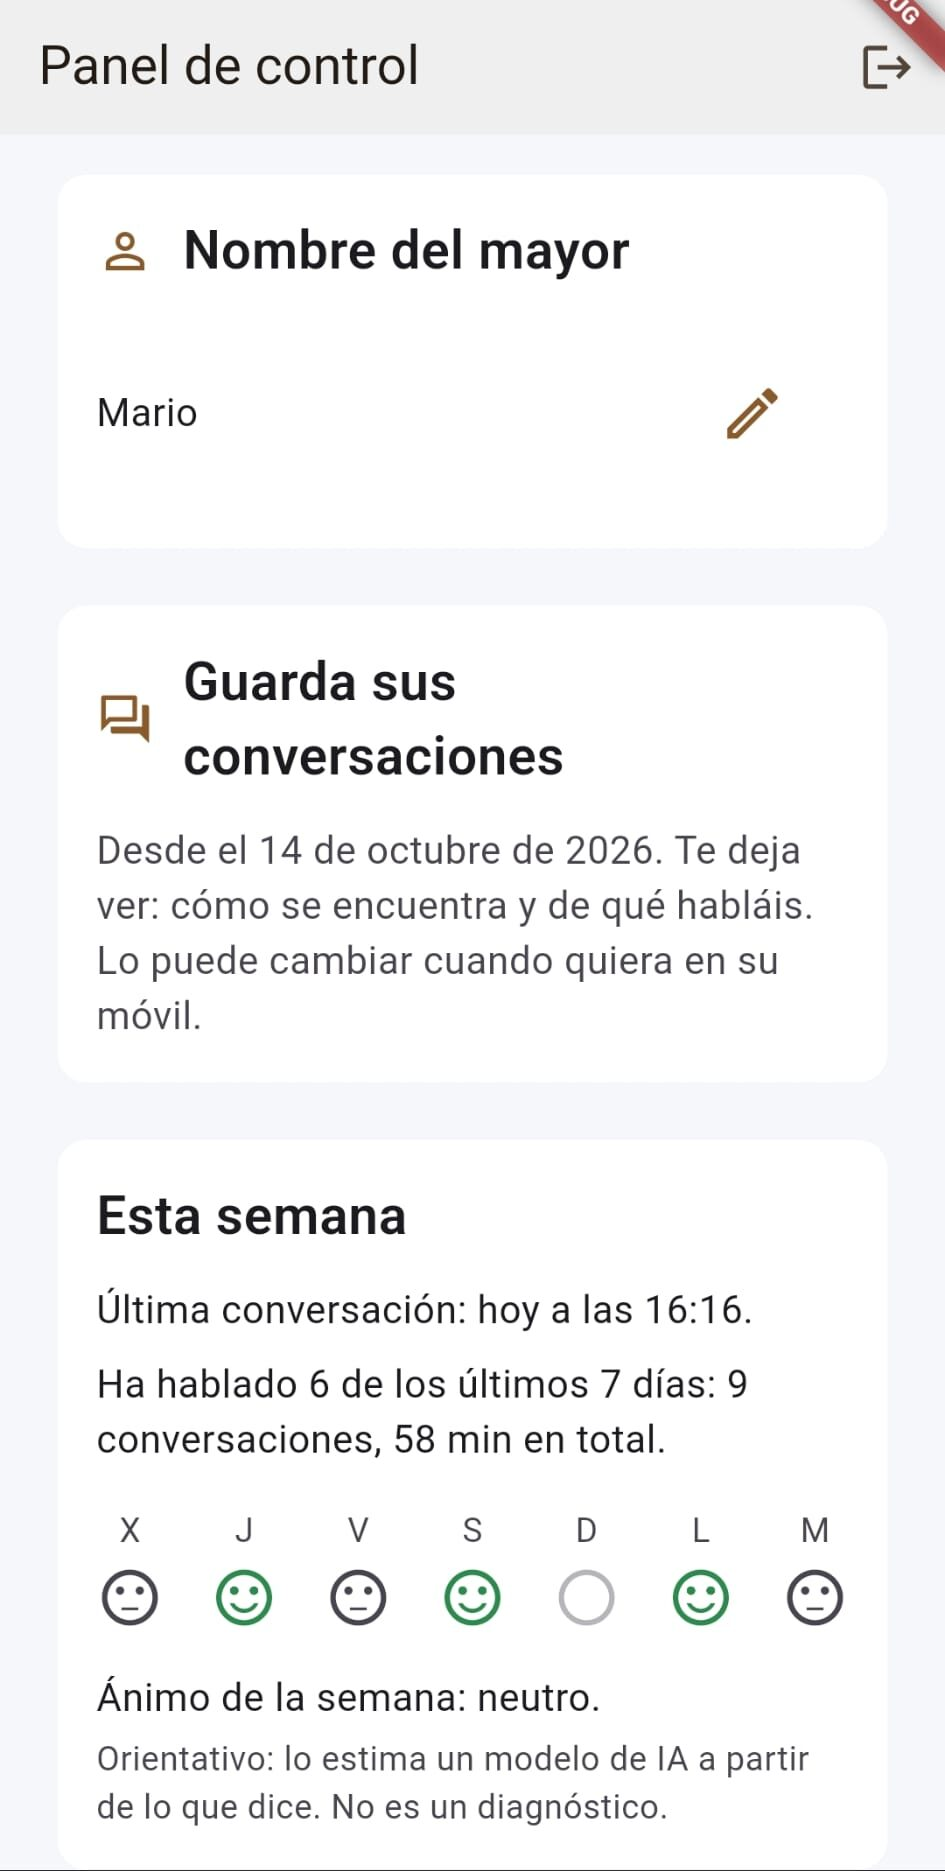
\includegraphics[width=\linewidth]{imagenes/manual/familiar-panel-semana}
    \caption{Esta semana}
  \end{subfigure}\hfill
  \begin{subfigure}[t]{0.27\textwidth}\centering
    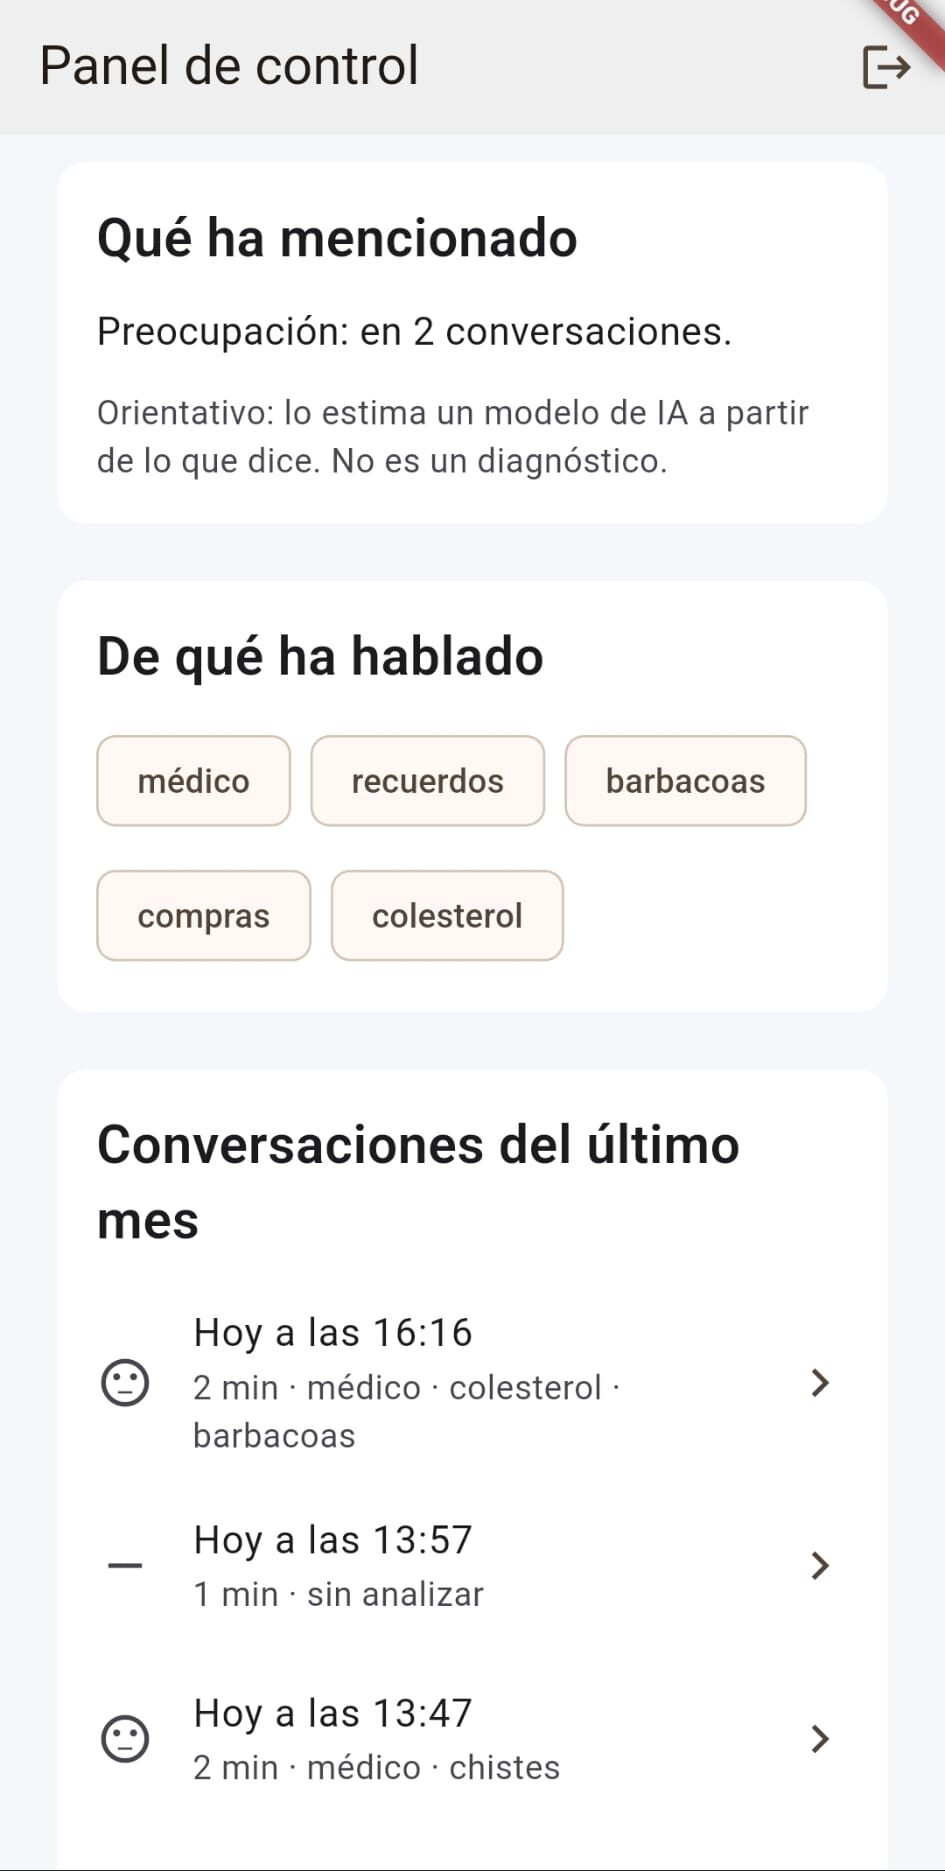
\includegraphics[width=\linewidth]{imagenes/manual/familiar-panel-temas}
    \caption{Señales y temas}
  \end{subfigure}\hfill
  \begin{subfigure}[t]{0.27\textwidth}\centering
    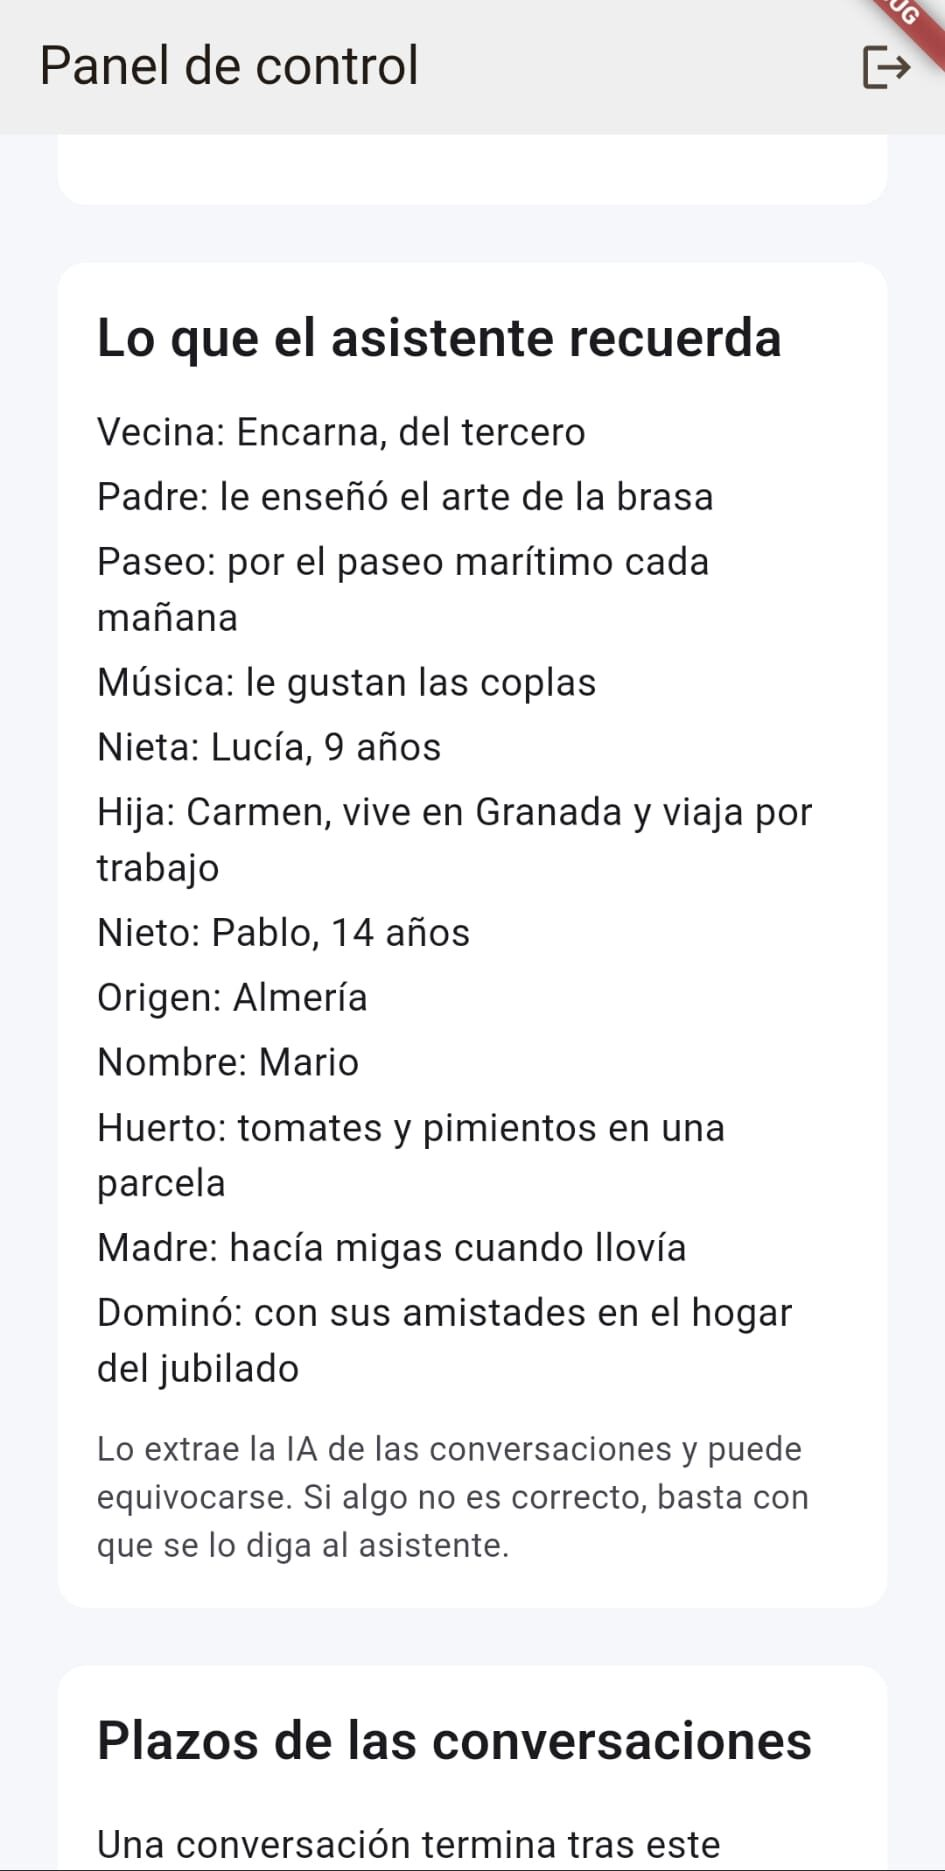
\includegraphics[width=\linewidth]{imagenes/manual/familiar-panel-recuerda}
    \caption{Lo que recuerda}
  \end{subfigure}
  \caption{Panel de control del familiar.}
  \label{fig:manual-panel}
\end{figure}

El panel es una sola pantalla que se recorre hacia abajo (\autoref{fig:manual-panel}). De arriba abajo muestra:

\begin{itemize}
  \item \textbf{Nombre del mayor.} El asistente lo aprende al conversar; el lápiz permite corregirlo.
  \item \textbf{Si guarda sus conversaciones}, desde cuándo y qué le deja ver. Solo la persona mayor puede cambiarlo, desde su móvil.
  \item \textbf{Esta semana.} Cuándo habló por última vez, cuántos días y cuánto tiempo, y una fila con los últimos siete días. La cara de cada día indica el ánimo (verde, positivo; gris, neutro; naranja, negativo), y el círculo vacío, que ese día no habló con el asistente.
  \item \textbf{Qué ha mencionado y de qué ha hablado.} Señales como preocupación, tristeza o soledad, con las conversaciones en que aparecen, y los temas que más se repiten.
  \item \textbf{Conversaciones del último mes.} Al tocar una se ve su detalle: cuándo fue, cuánto duró, el ánimo, lo que mencionó, un resumen breve y los temas. Las marcadas <<sin analizar>> no tienen resumen.
  \item \textbf{Lo que el asistente recuerda.} Lo que la persona mayor le ha contado de sí misma, como su familia o sus aficiones. Si algo no es correcto, basta con que ella se lo diga al asistente.
\end{itemize}

Si la persona mayor solo comparte <<Cómo me encuentro>>, no se muestran los temas, los resúmenes ni lo que recuerda el asistente, y en ningún caso se ve lo que dijo palabra por palabra. El ánimo y las señales los estima un modelo de inteligencia artificial: son orientativos, no un diagnóstico. Si en alguna conversación de la semana habló de hacerse daño o de no querer vivir, el panel lo avisa arriba, en rojo, junto a los teléfonos 112 y 024.

Al final del panel se fijan los plazos: cuánto silencio da por terminada una conversación (de 2 a 15 minutos) y cuánto se guarda cada resumen (de 1 a 6 meses); si acorta este último, lo que quede fuera se borra tras la siguiente conversación. En <<Preferencias de voz y texto>> elige la voz del asistente (el botón de reproducir la deja oír) y ajusta el volumen, la velocidad del habla y el tamaño del texto en el móvil de la persona mayor, que recibe los cambios al momento. Para cerrar sesión, use el icono de arriba a la derecha.
